\documentclass{beamer}
\usepackage{graphicx}
\usepackage{tikz}
\usetikzlibrary{shapes,arrows}
\usepackage{tikz}
%\usecolortheme{seahorse}
  \setbeamertemplate{footline}[page number]
\usepackage{multirow}
\setbeamertemplate{navigation symbols}{}
\setbeamertemplate{frametitle}[default][center]
\setbeamerfont{frametitle}{shape=\scshape}
\usepackage{color}

\usepackage{csquotes}

\usepackage{xcolor}

\usepackage[flushleft]{threeparttable}

{\title{\textsc{Econ 352 - Business Cycle Measurement} \\ \tiny (See Williamson Ch. 3)}
\author{Trevor S. Gallen}
\date{}
\begin{document}
\renewcommand*{\inserttotalframenumber}{\pageref{lastframe}}


\setbeamertemplate{caption}{\raggedright\insertcaption\par}

\begin{frame}
\titlepage
\end{frame}

\begin{frame}
\frametitle[alignment=center]{Measuring Business Cycles}
\begin{itemize}
\item In this lecture we'll think about how deviations of GDP from trend \textcolor{red}{and the things that co-move with it}
\bigskip
\item Explaining the co-movements is key: constrains theory space sharply!
\bigskip
\item Note:  my \#'s will deviate from Williamson's because I'll be using a different filter, but lessons are same
\end{itemize}
\end{frame}


\begin{frame}
\frametitle[alignment=center]{Measuring Business Cycles}
\begin{itemize}
\item In this lecture we'll think about how deviations of GDP from trend \textcolor{red}{and the things that co-move with it}
\bigskip
\item Explaining the co-movements is key: constrains theory space sharply!
\bigskip
\item Lesson for life:  whenever you create a hypothesis to explain X, thinking of side predictions on Y and Z (that you didn't create the model to explain, but it has opinions on) is a very valuable practice!
\end{itemize}
\end{frame}

\begin{frame}
\frametitle[alignment=center]{Idealized Business Cycle}
\begin{figure}
\centering
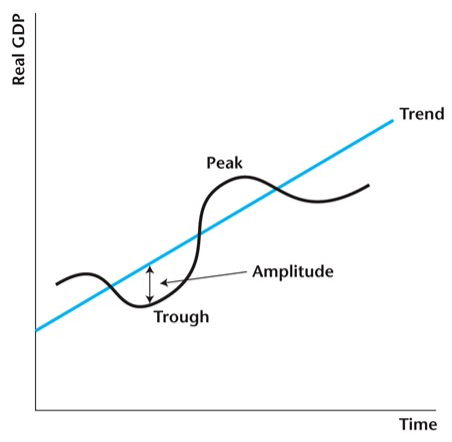
\includegraphics[scale=0.7]{Figures/W_Fig_3pt1.png}
\end{figure}
\end{frame}



\begin{frame}
\frametitle[alignment=center]{Real GDP Deviations}
\begin{figure}
\centering
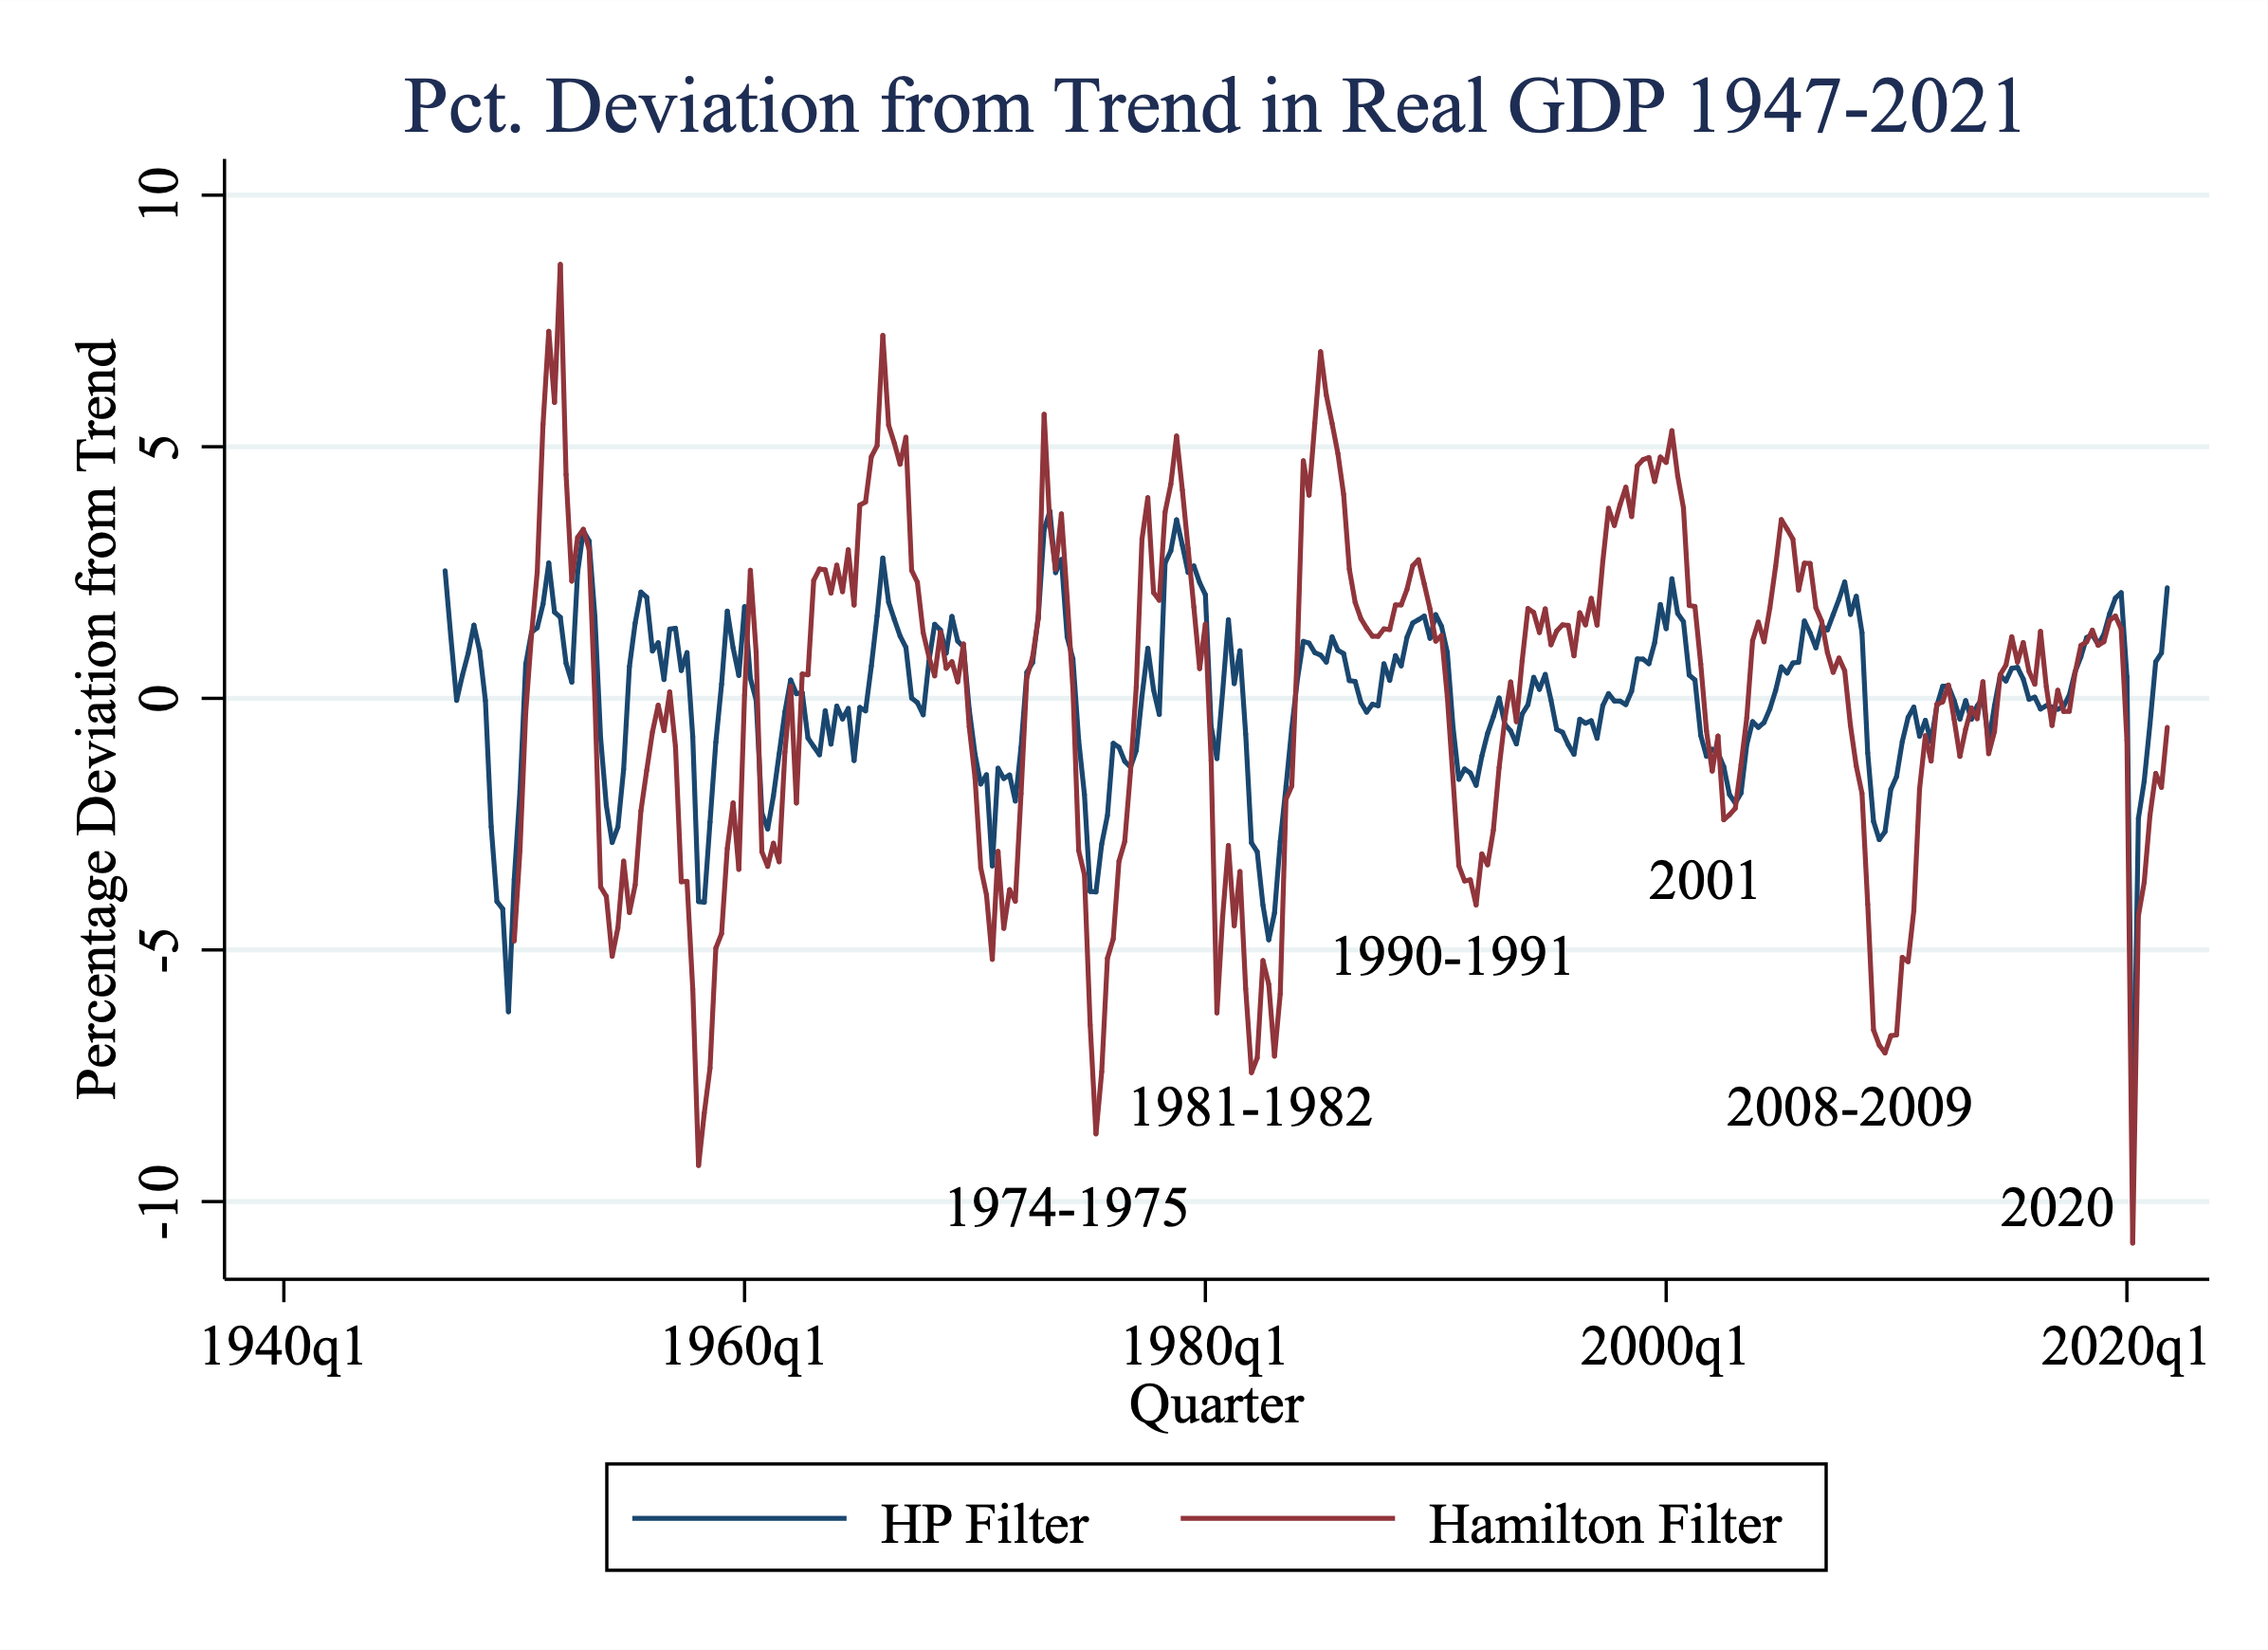
\includegraphics[scale=0.25]{Figures/Fig_3pt2.png}
\end{figure}
Takeaways:  deviations are persistent, magnitudes are a few years of growth at most
\end{frame}

\begin{frame}
\frametitle[alignment=center]{Positive vs Negative Comovement}
\begin{figure}
\centering
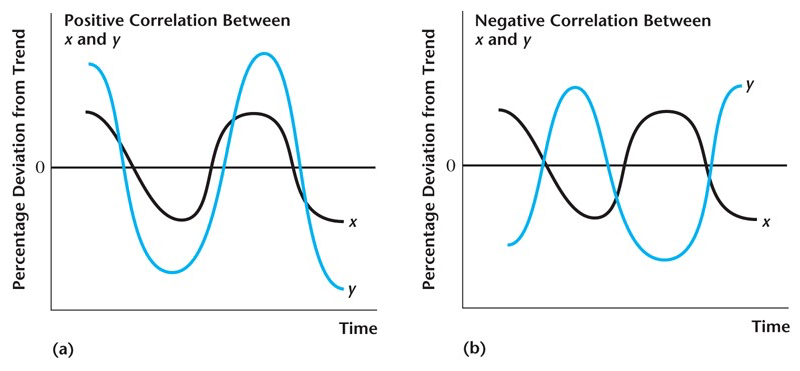
\includegraphics[scale=0.5]{Figures/W_Fig_3pt3.png}
\end{figure}
\end{frame}

\begin{frame}
\frametitle[alignment=center]{HotSeat Question!}
\begin{itemize}
\item Is the price level pro-, a-, or countercyclical?
\end{itemize}
\end{frame}


\begin{frame}
\frametitle[alignment=center]{Cyclicality}
\begin{itemize}
\item If something moves with GDP (cyclically) then it's \textbf{procyclical} (like employment)
\item If something moves the opposite direction of GDP (cyclically) then it's \textbf{countercyclical} (like unemployment)
\item If something doesn't move with GDP then it's \textbf{acyclical} 
\end{itemize}
\end{frame}


\begin{frame}
\frametitle[alignment=center]{Imports and Real GDP}
\begin{figure}
\centering
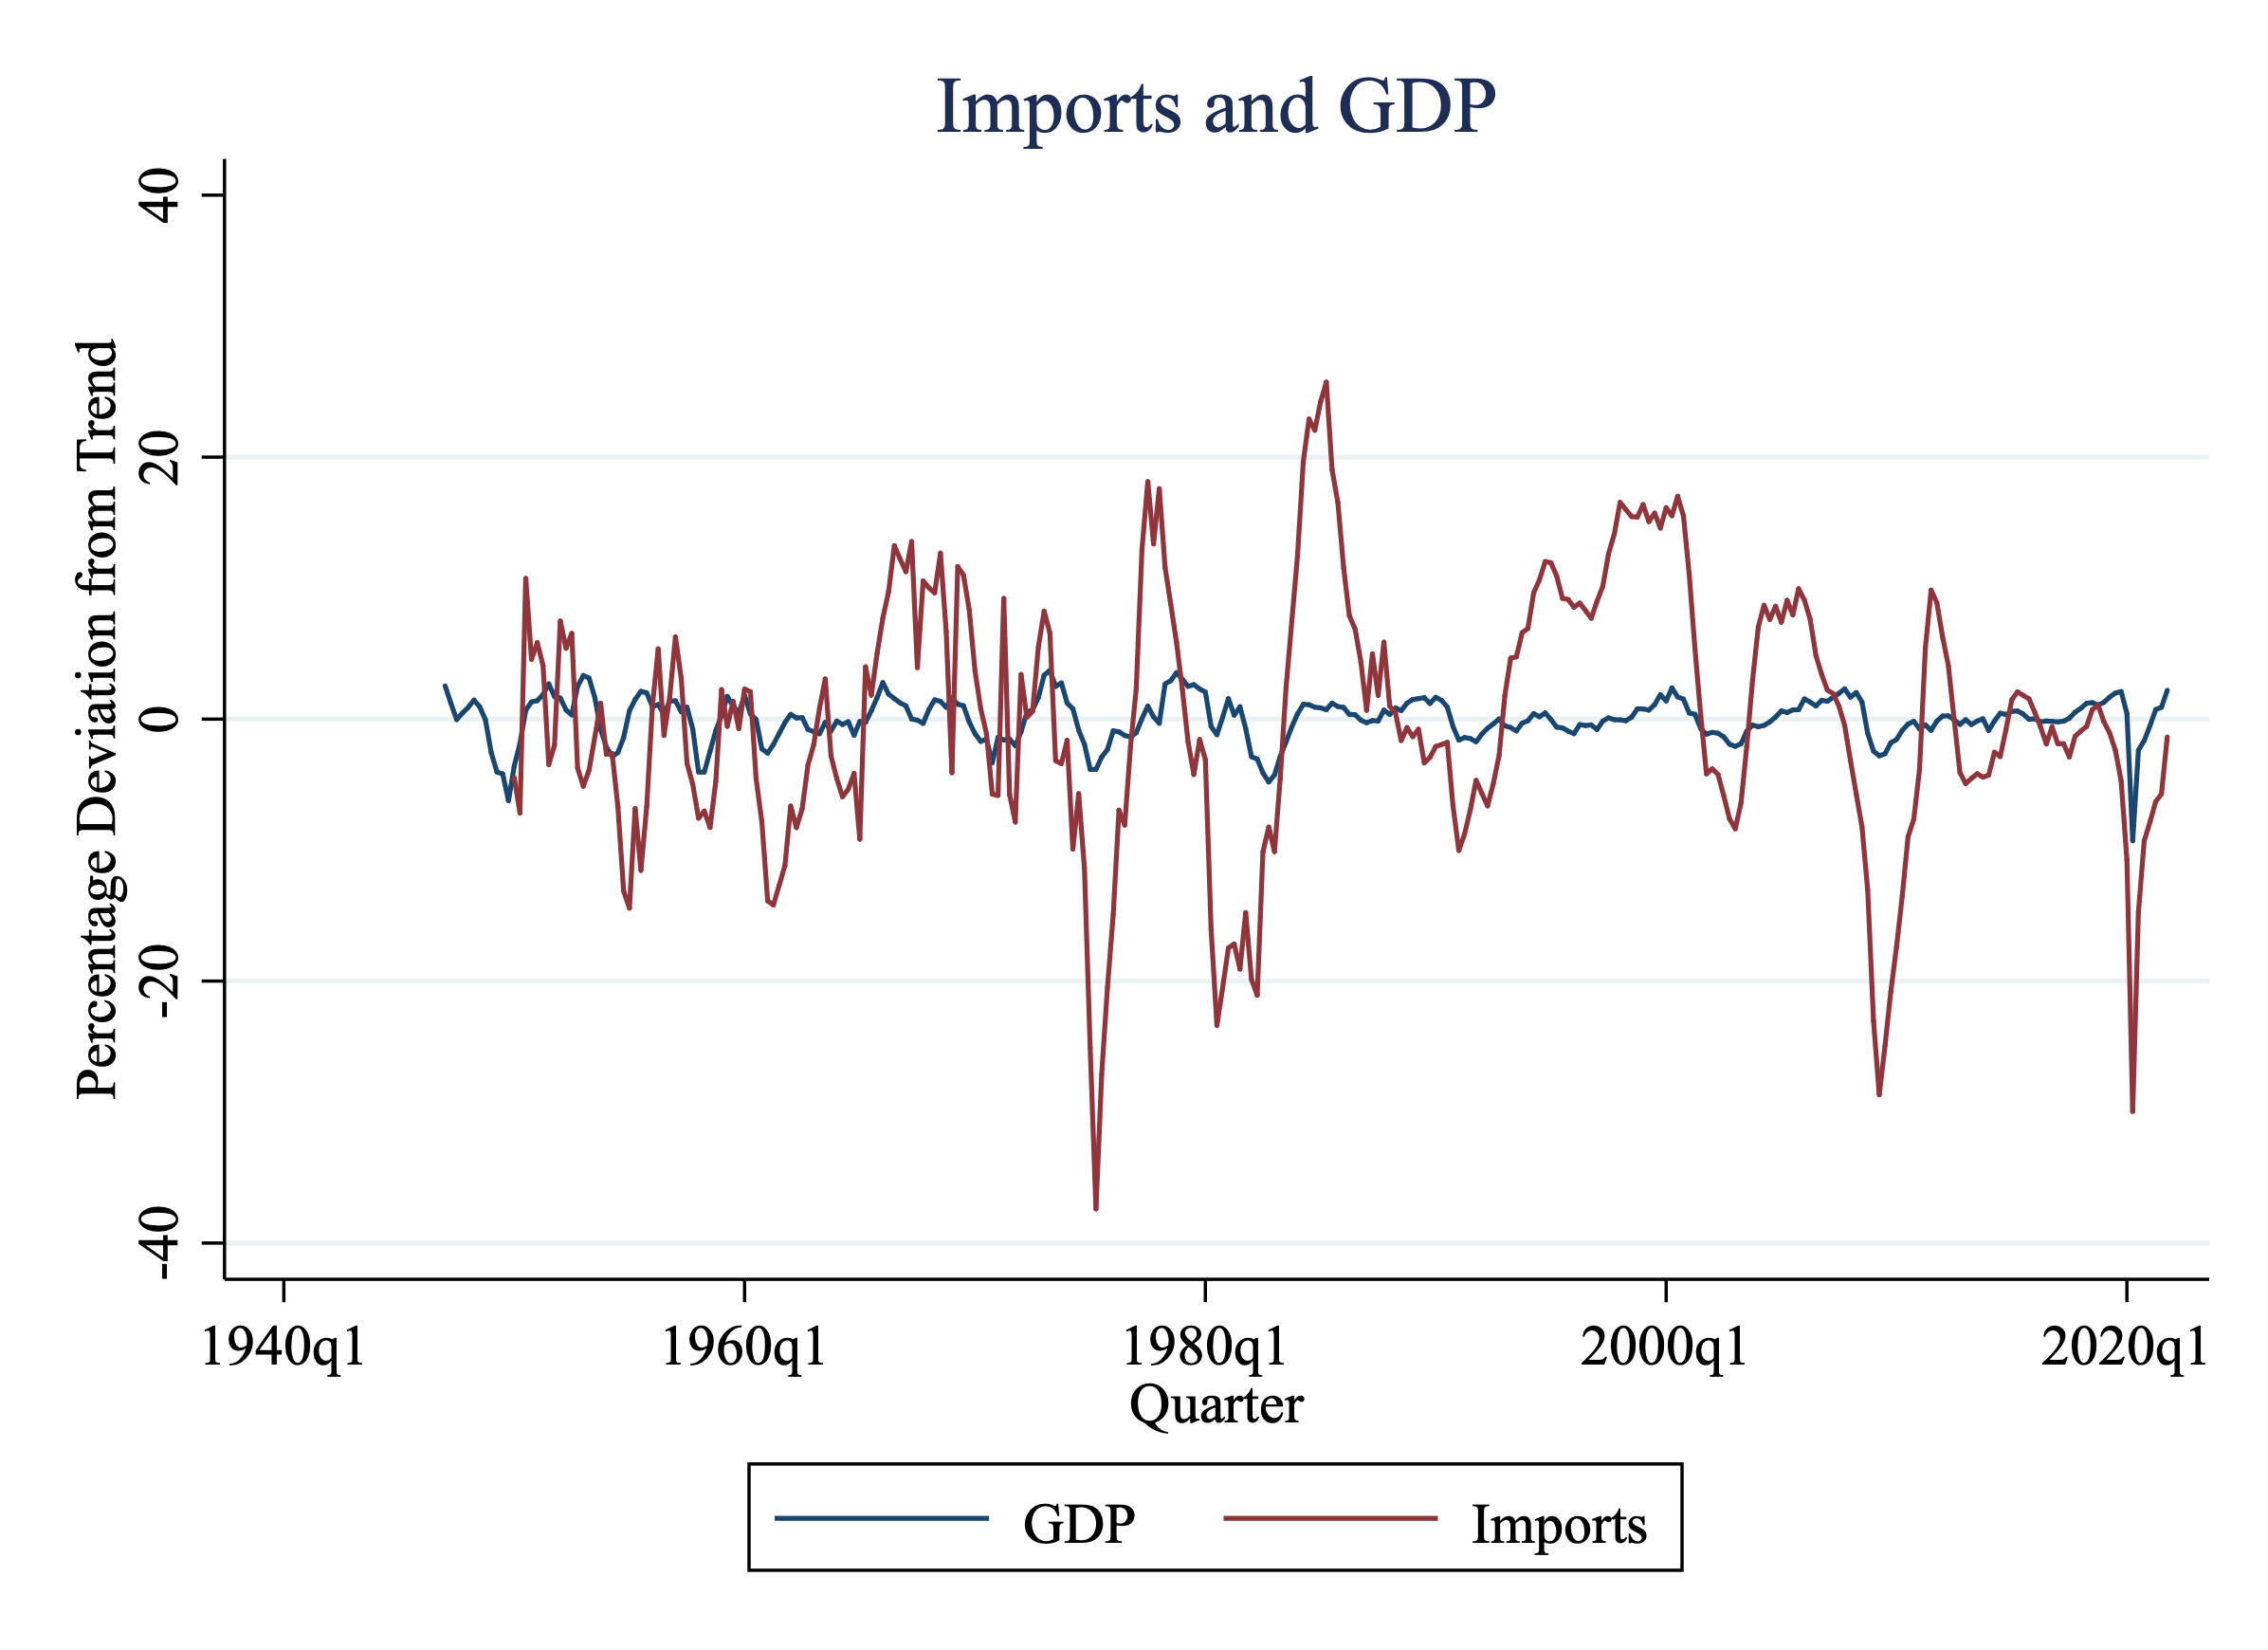
\includegraphics[scale=0.25]{Figures/Fig_3pt5.png}
\end{figure}
\end{frame}

\begin{frame}
\frametitle[alignment=center]{Imports and Real GDP}
\begin{figure}
\centering
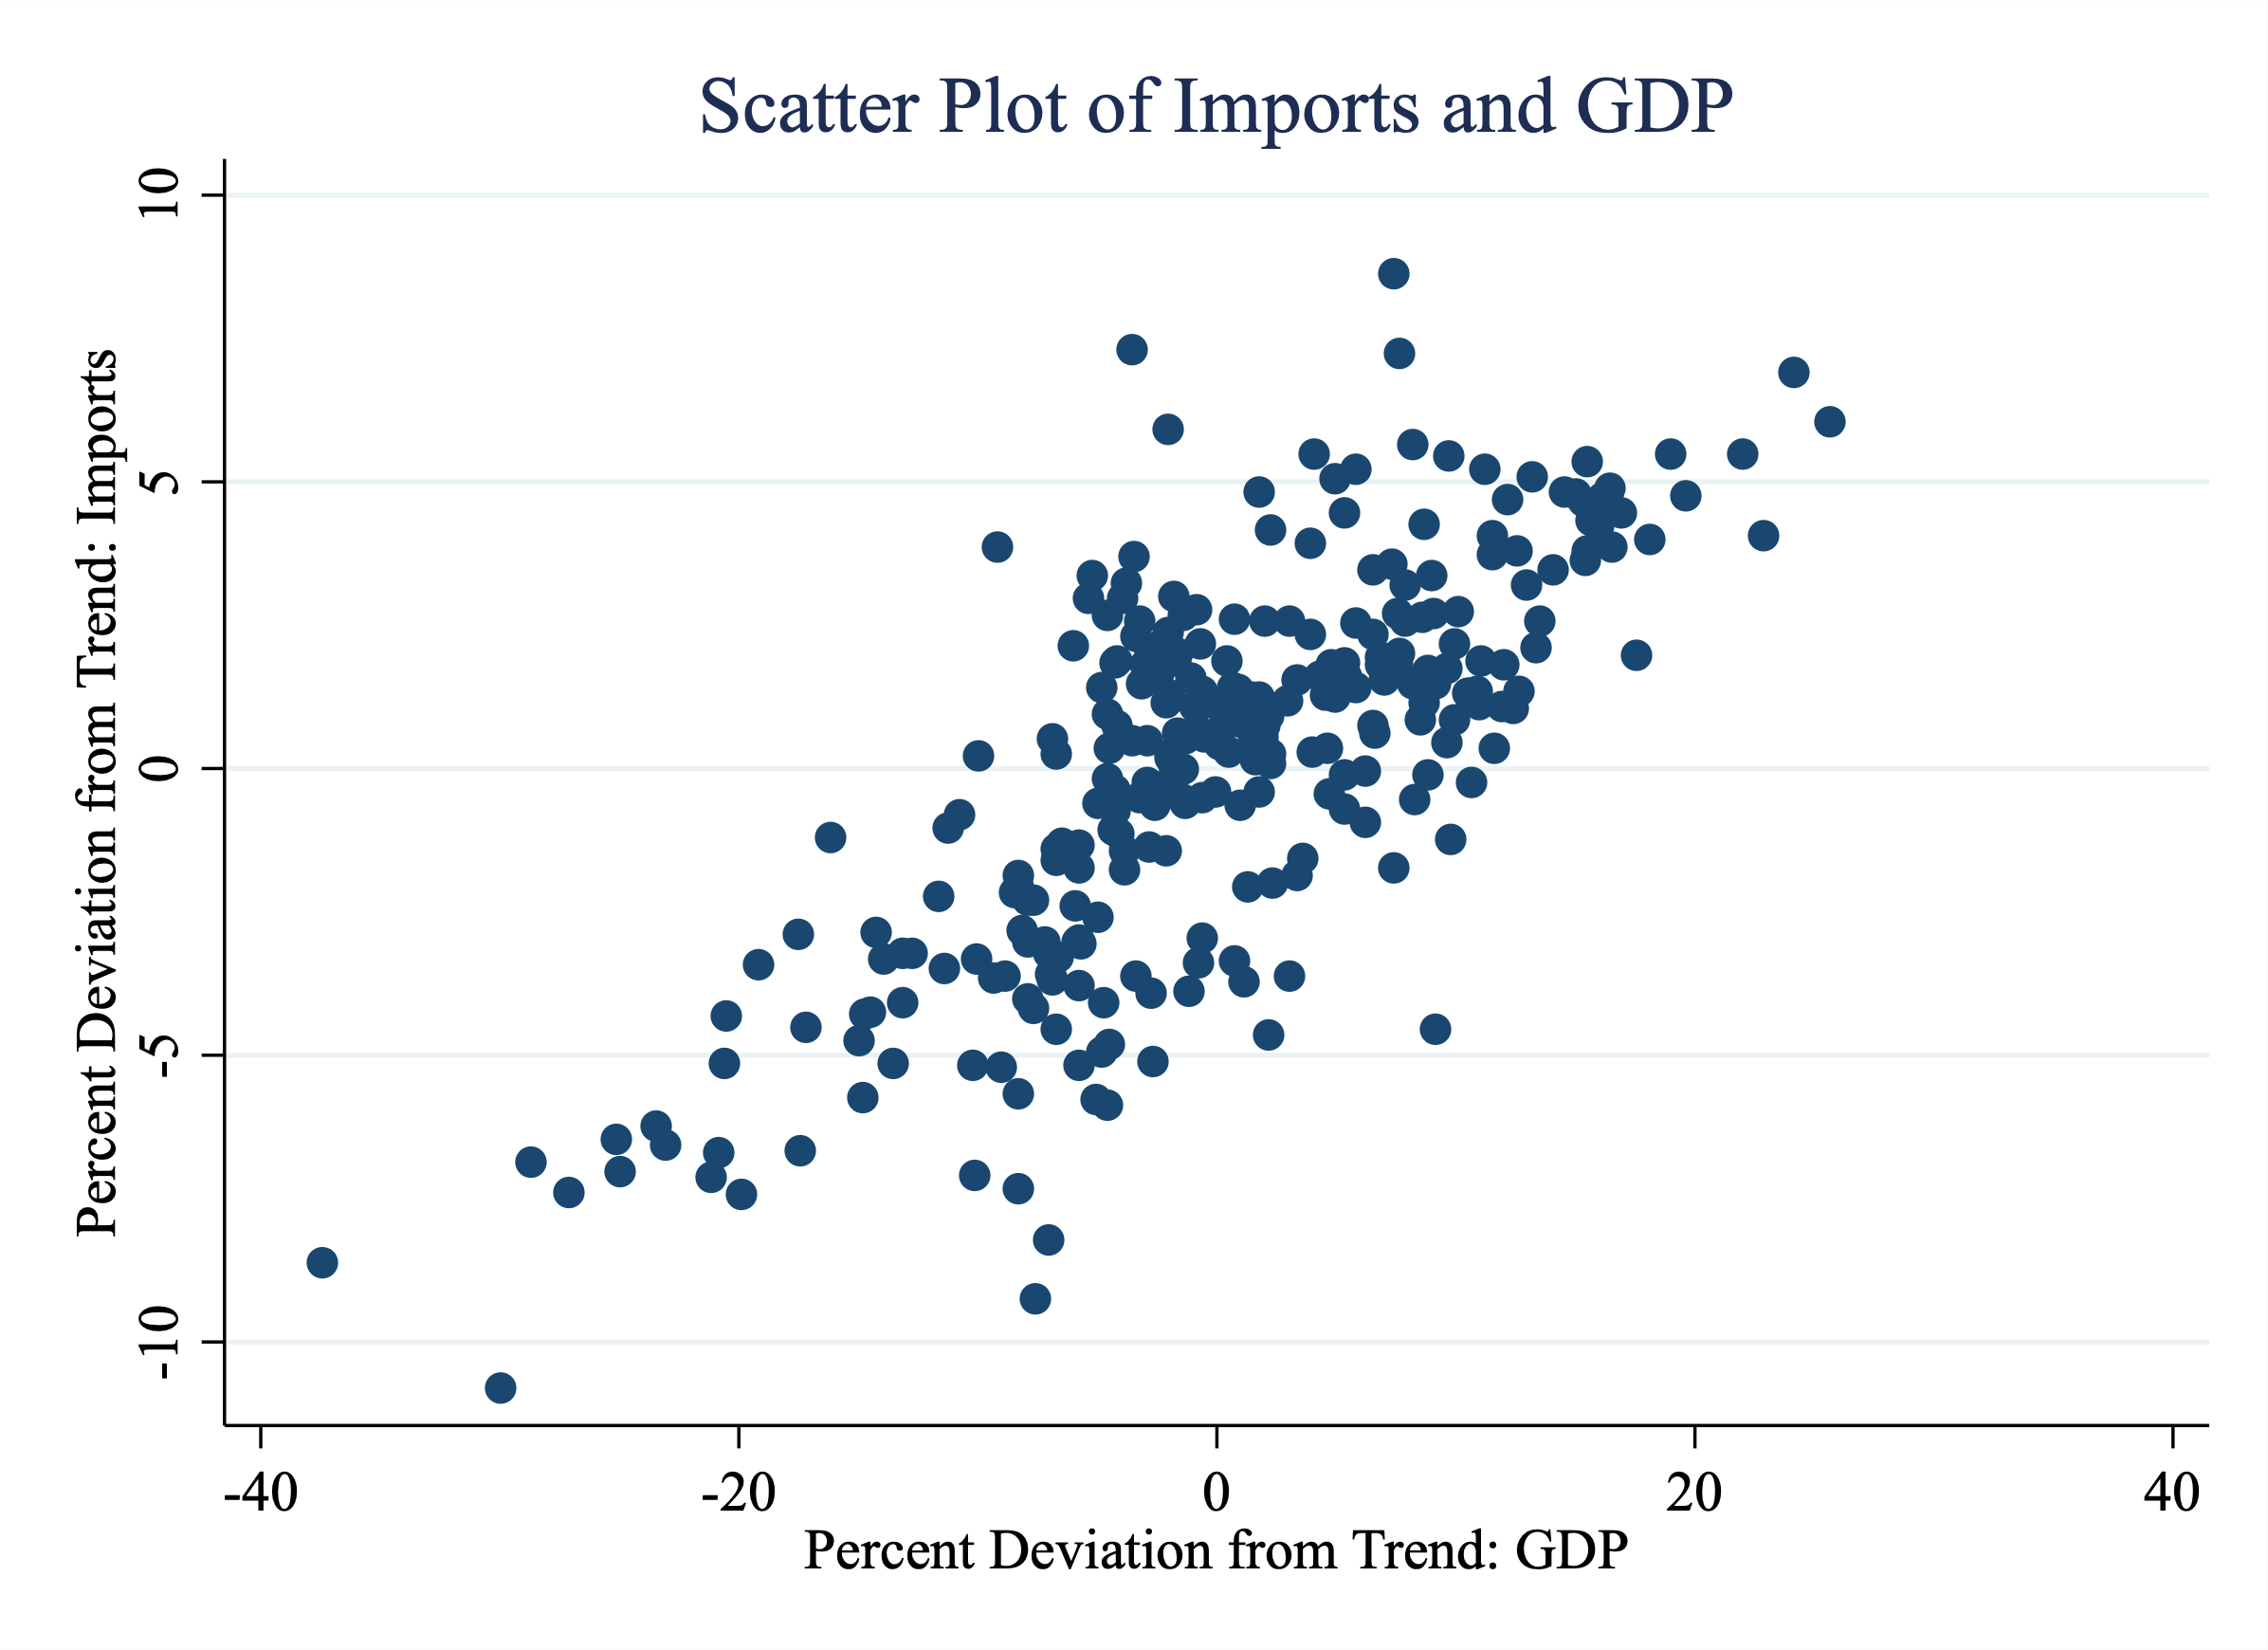
\includegraphics[scale=0.25]{Figures/Fig_3pt6.png}
\end{figure}
\end{frame}

\begin{frame}
\frametitle[alignment=center]{Lags vs Leads}
\begin{figure}
\centering
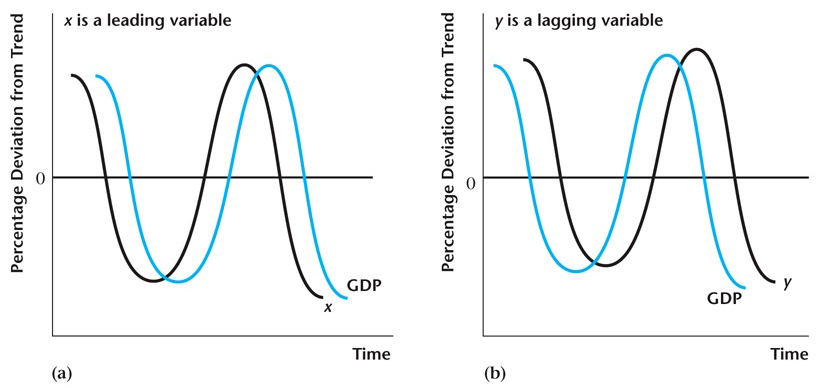
\includegraphics[scale=0.5]{Figures/W_Fig_3pt7.png}
\end{figure}
\end{frame}


\begin{frame}
\frametitle[alignment=center]{Housing and Real GDP}
\begin{figure}
\centering
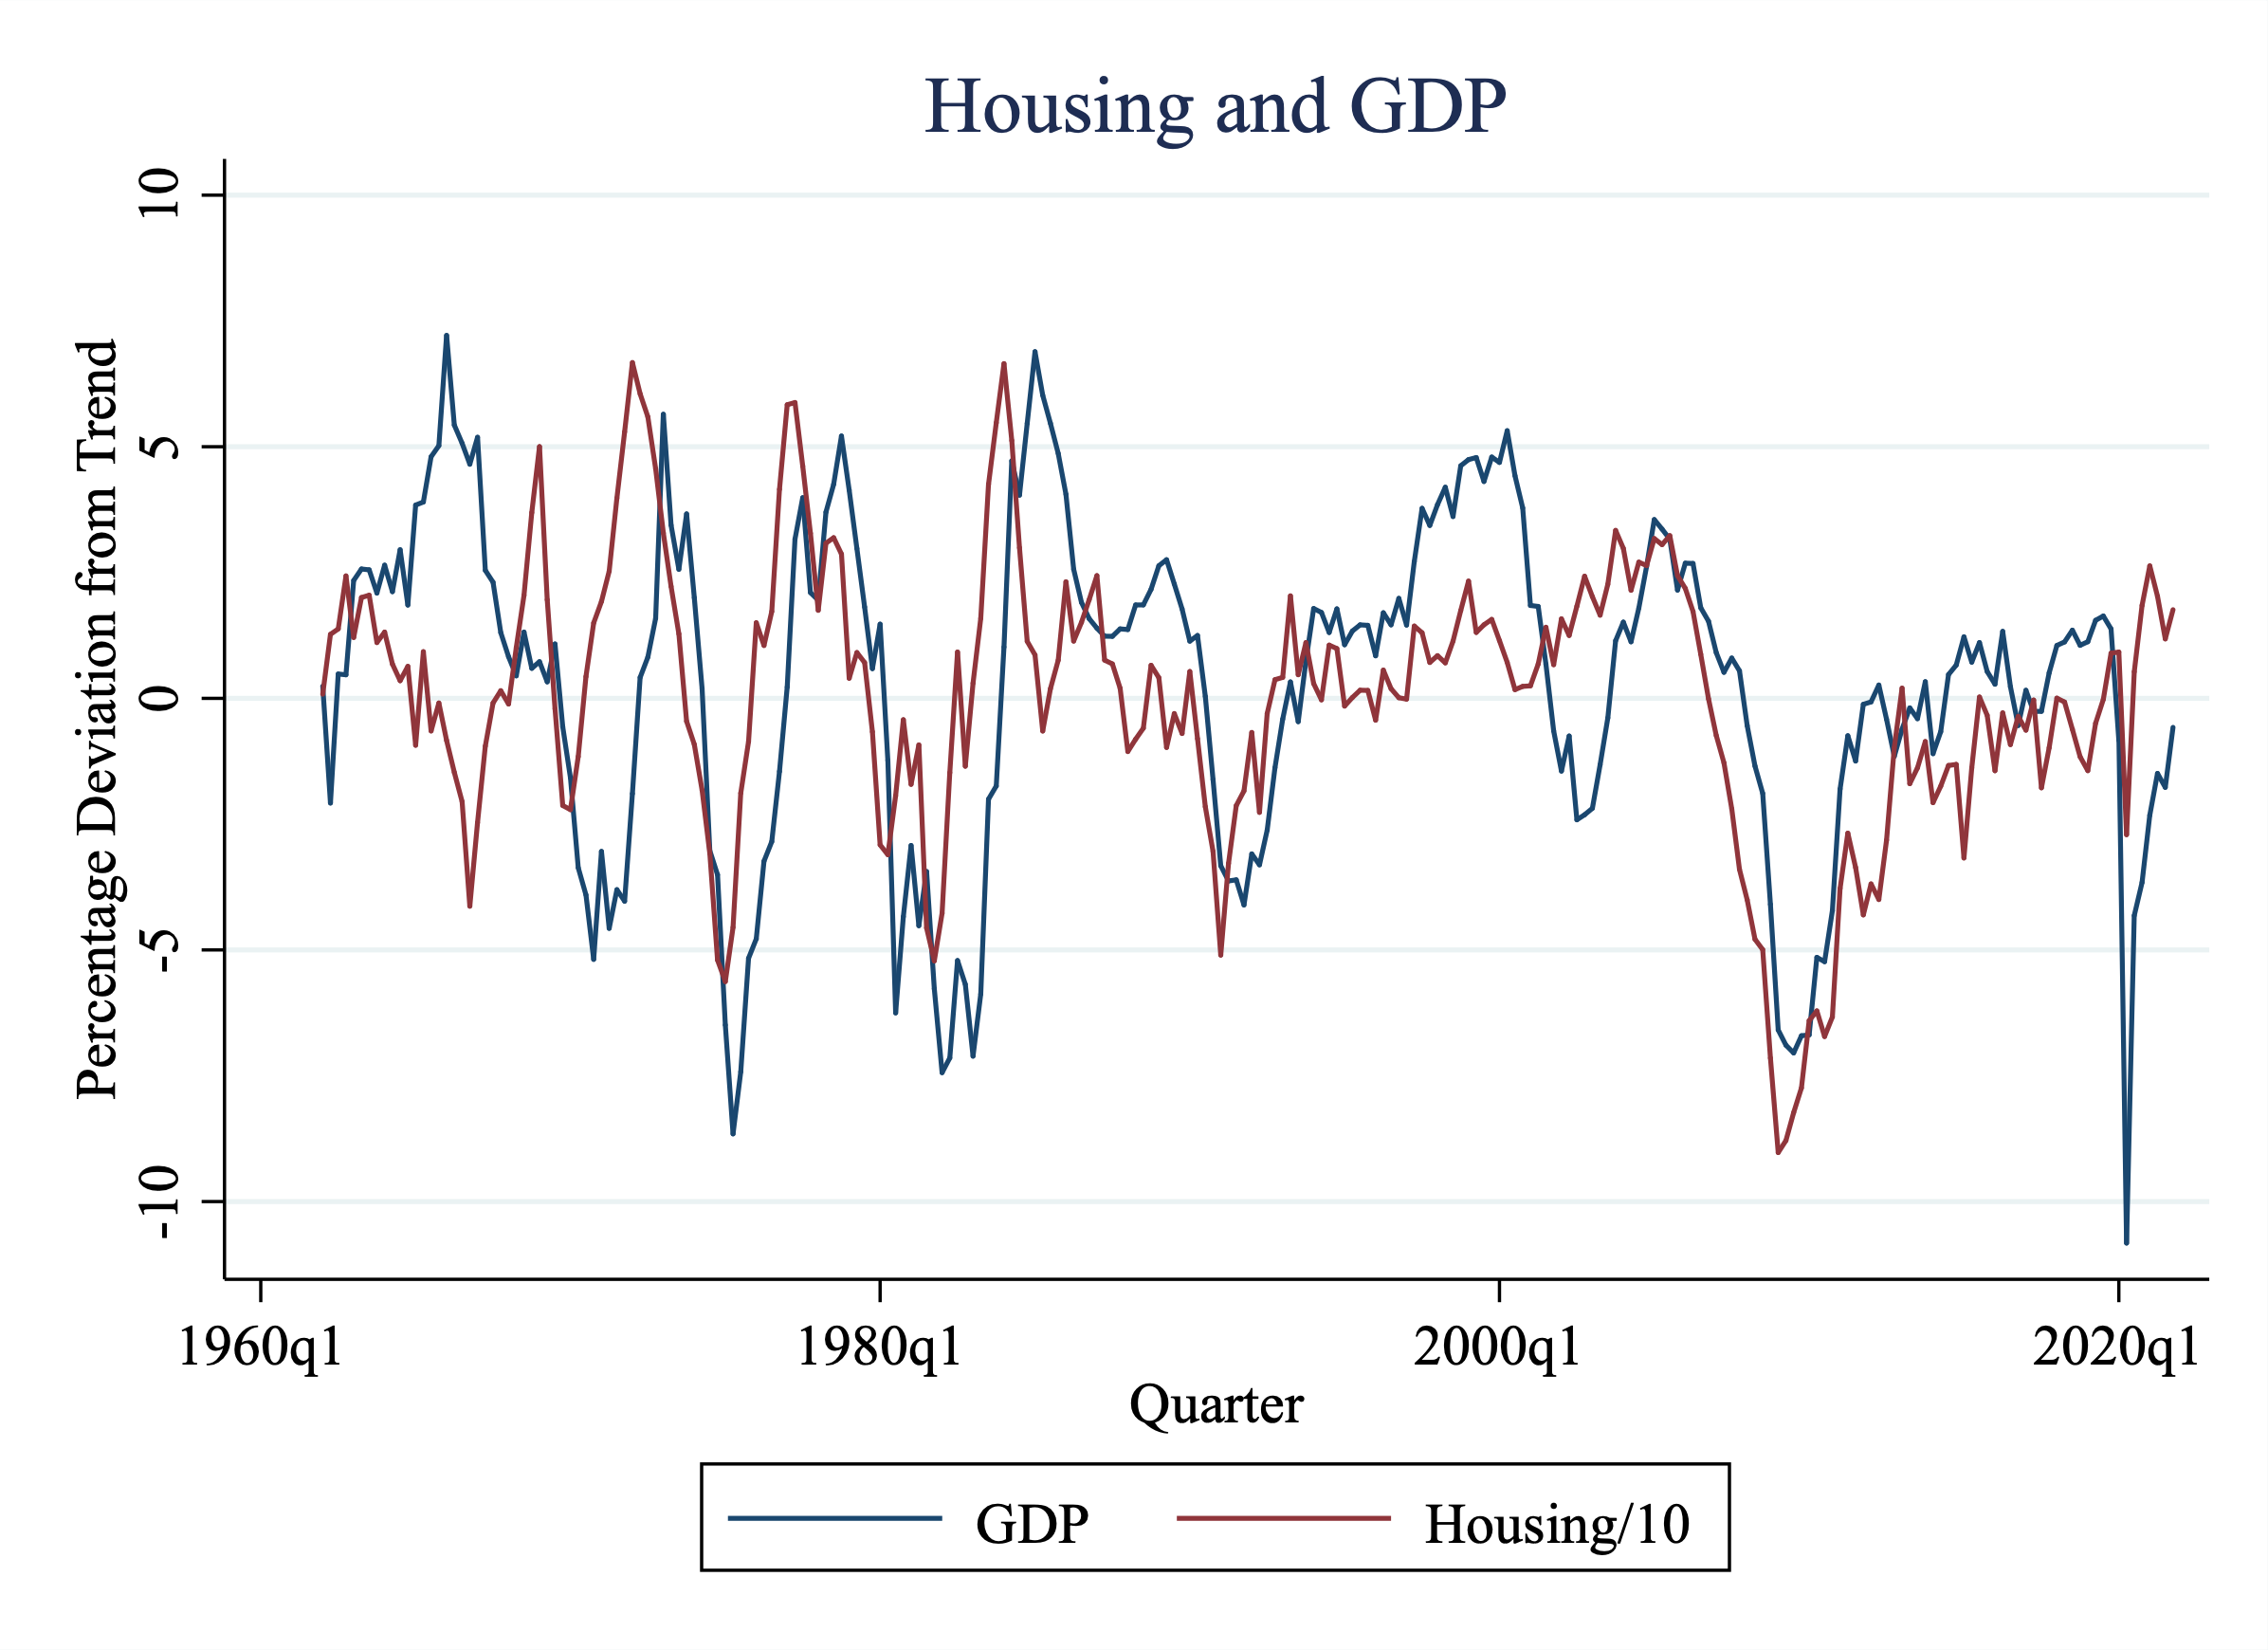
\includegraphics[scale=0.25]{Figures/Fig_3pt8.png}
\end{figure}
\end{frame}

\begin{frame}
\frametitle[alignment=center]{Consumption and Real GDP}
\begin{figure}
\centering
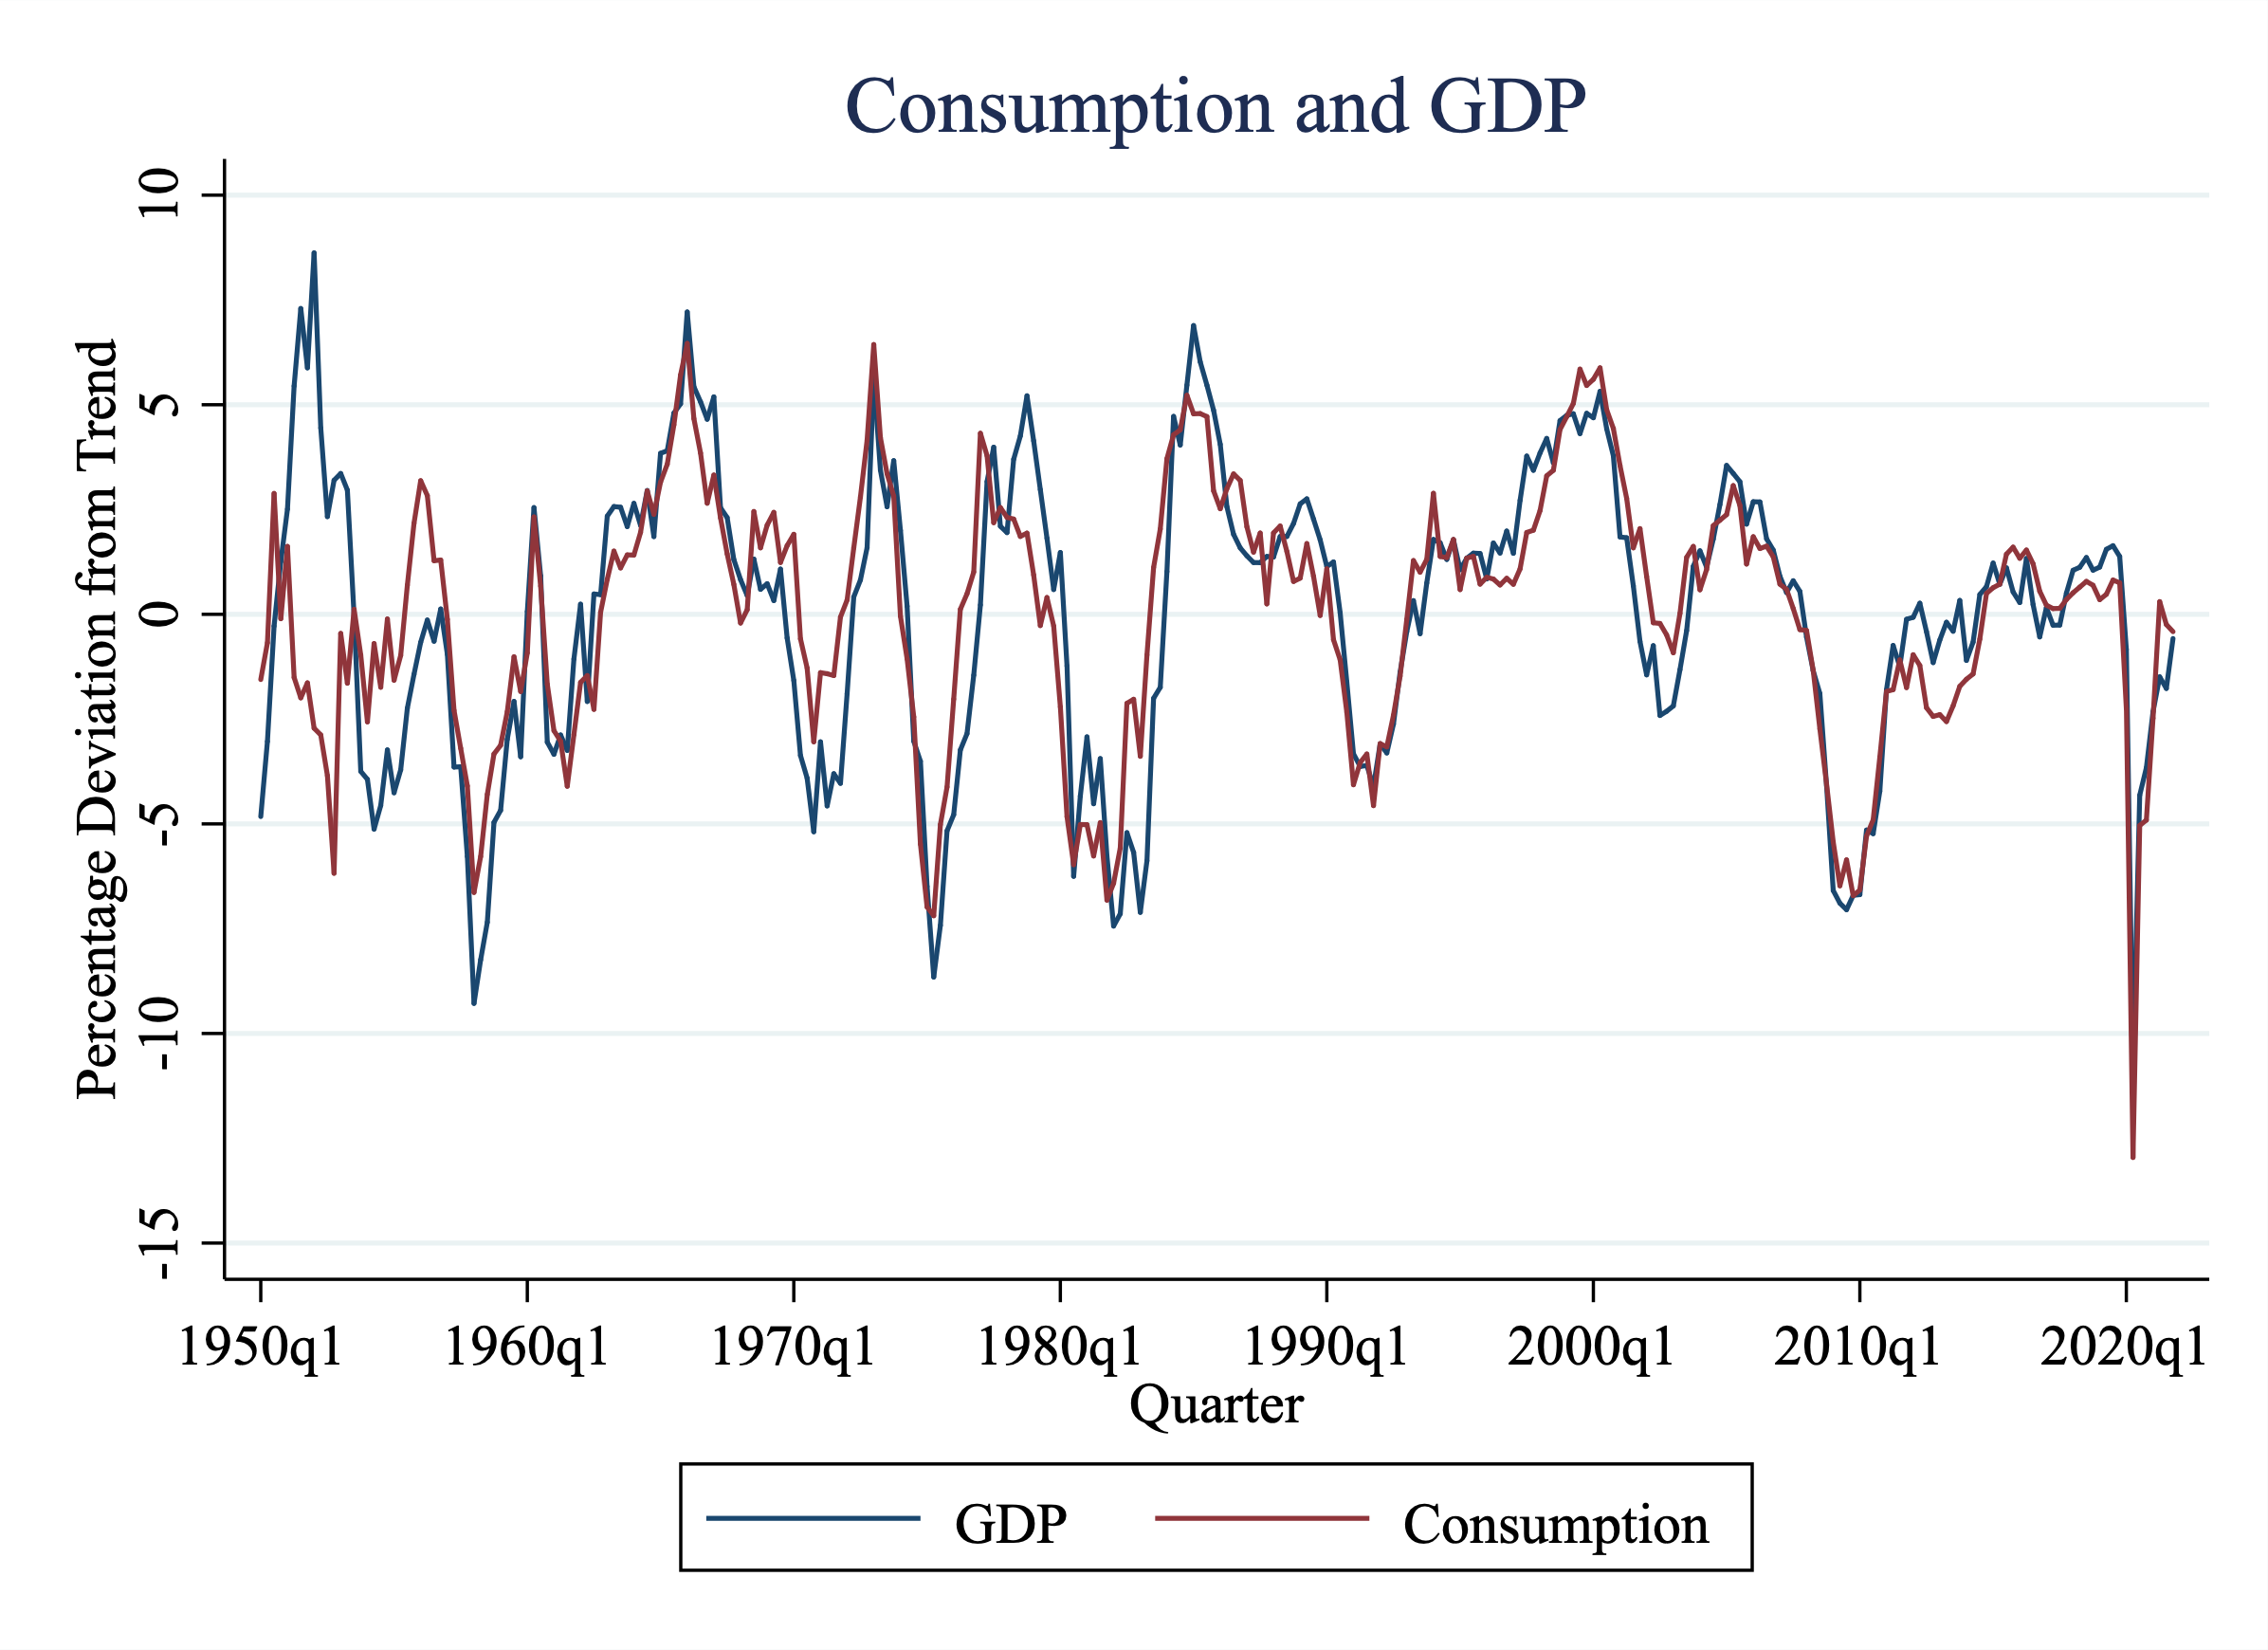
\includegraphics[scale=0.25]{Figures/Fig_3pt9.png}
\end{figure}
\end{frame}

\begin{frame}
\frametitle[alignment=center]{Investment and Real GDP}
\begin{figure}
\centering
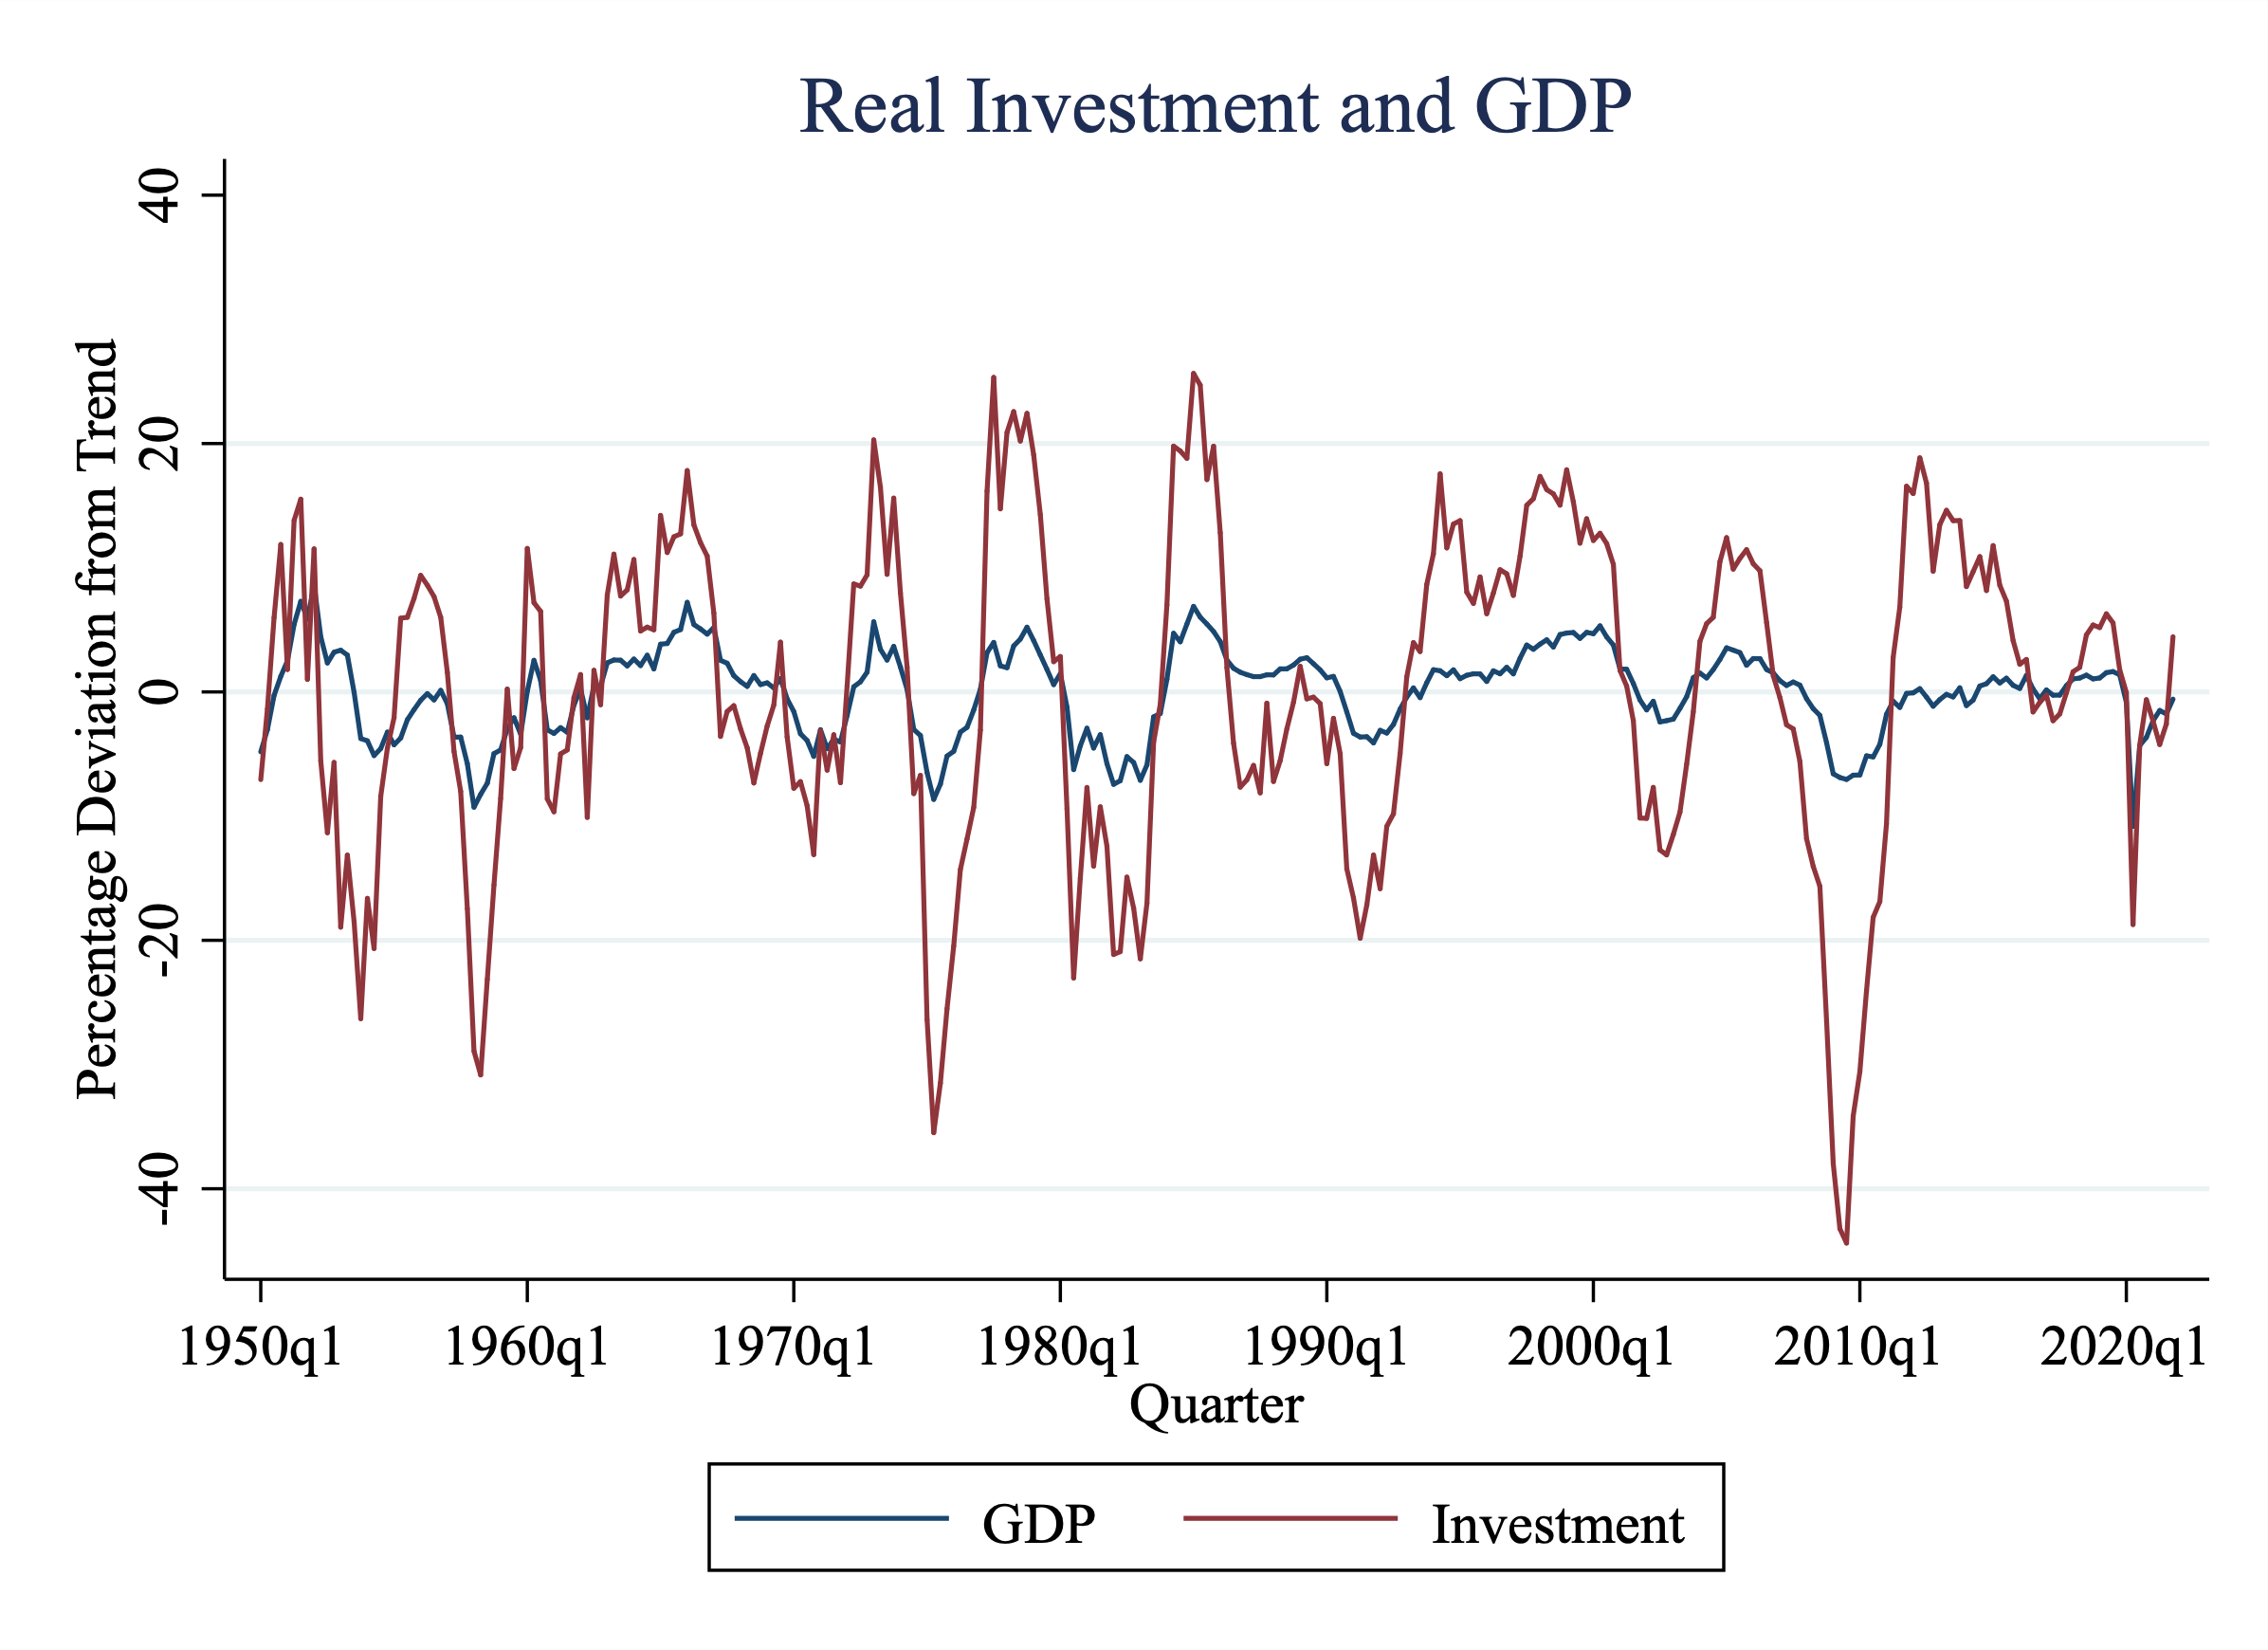
\includegraphics[scale=0.25]{Figures/Fig_3pt10.png}
\end{figure}
\end{frame}


\begin{frame}
\frametitle[alignment=center]{Price Level and Real GDP}
\begin{figure}
\centering
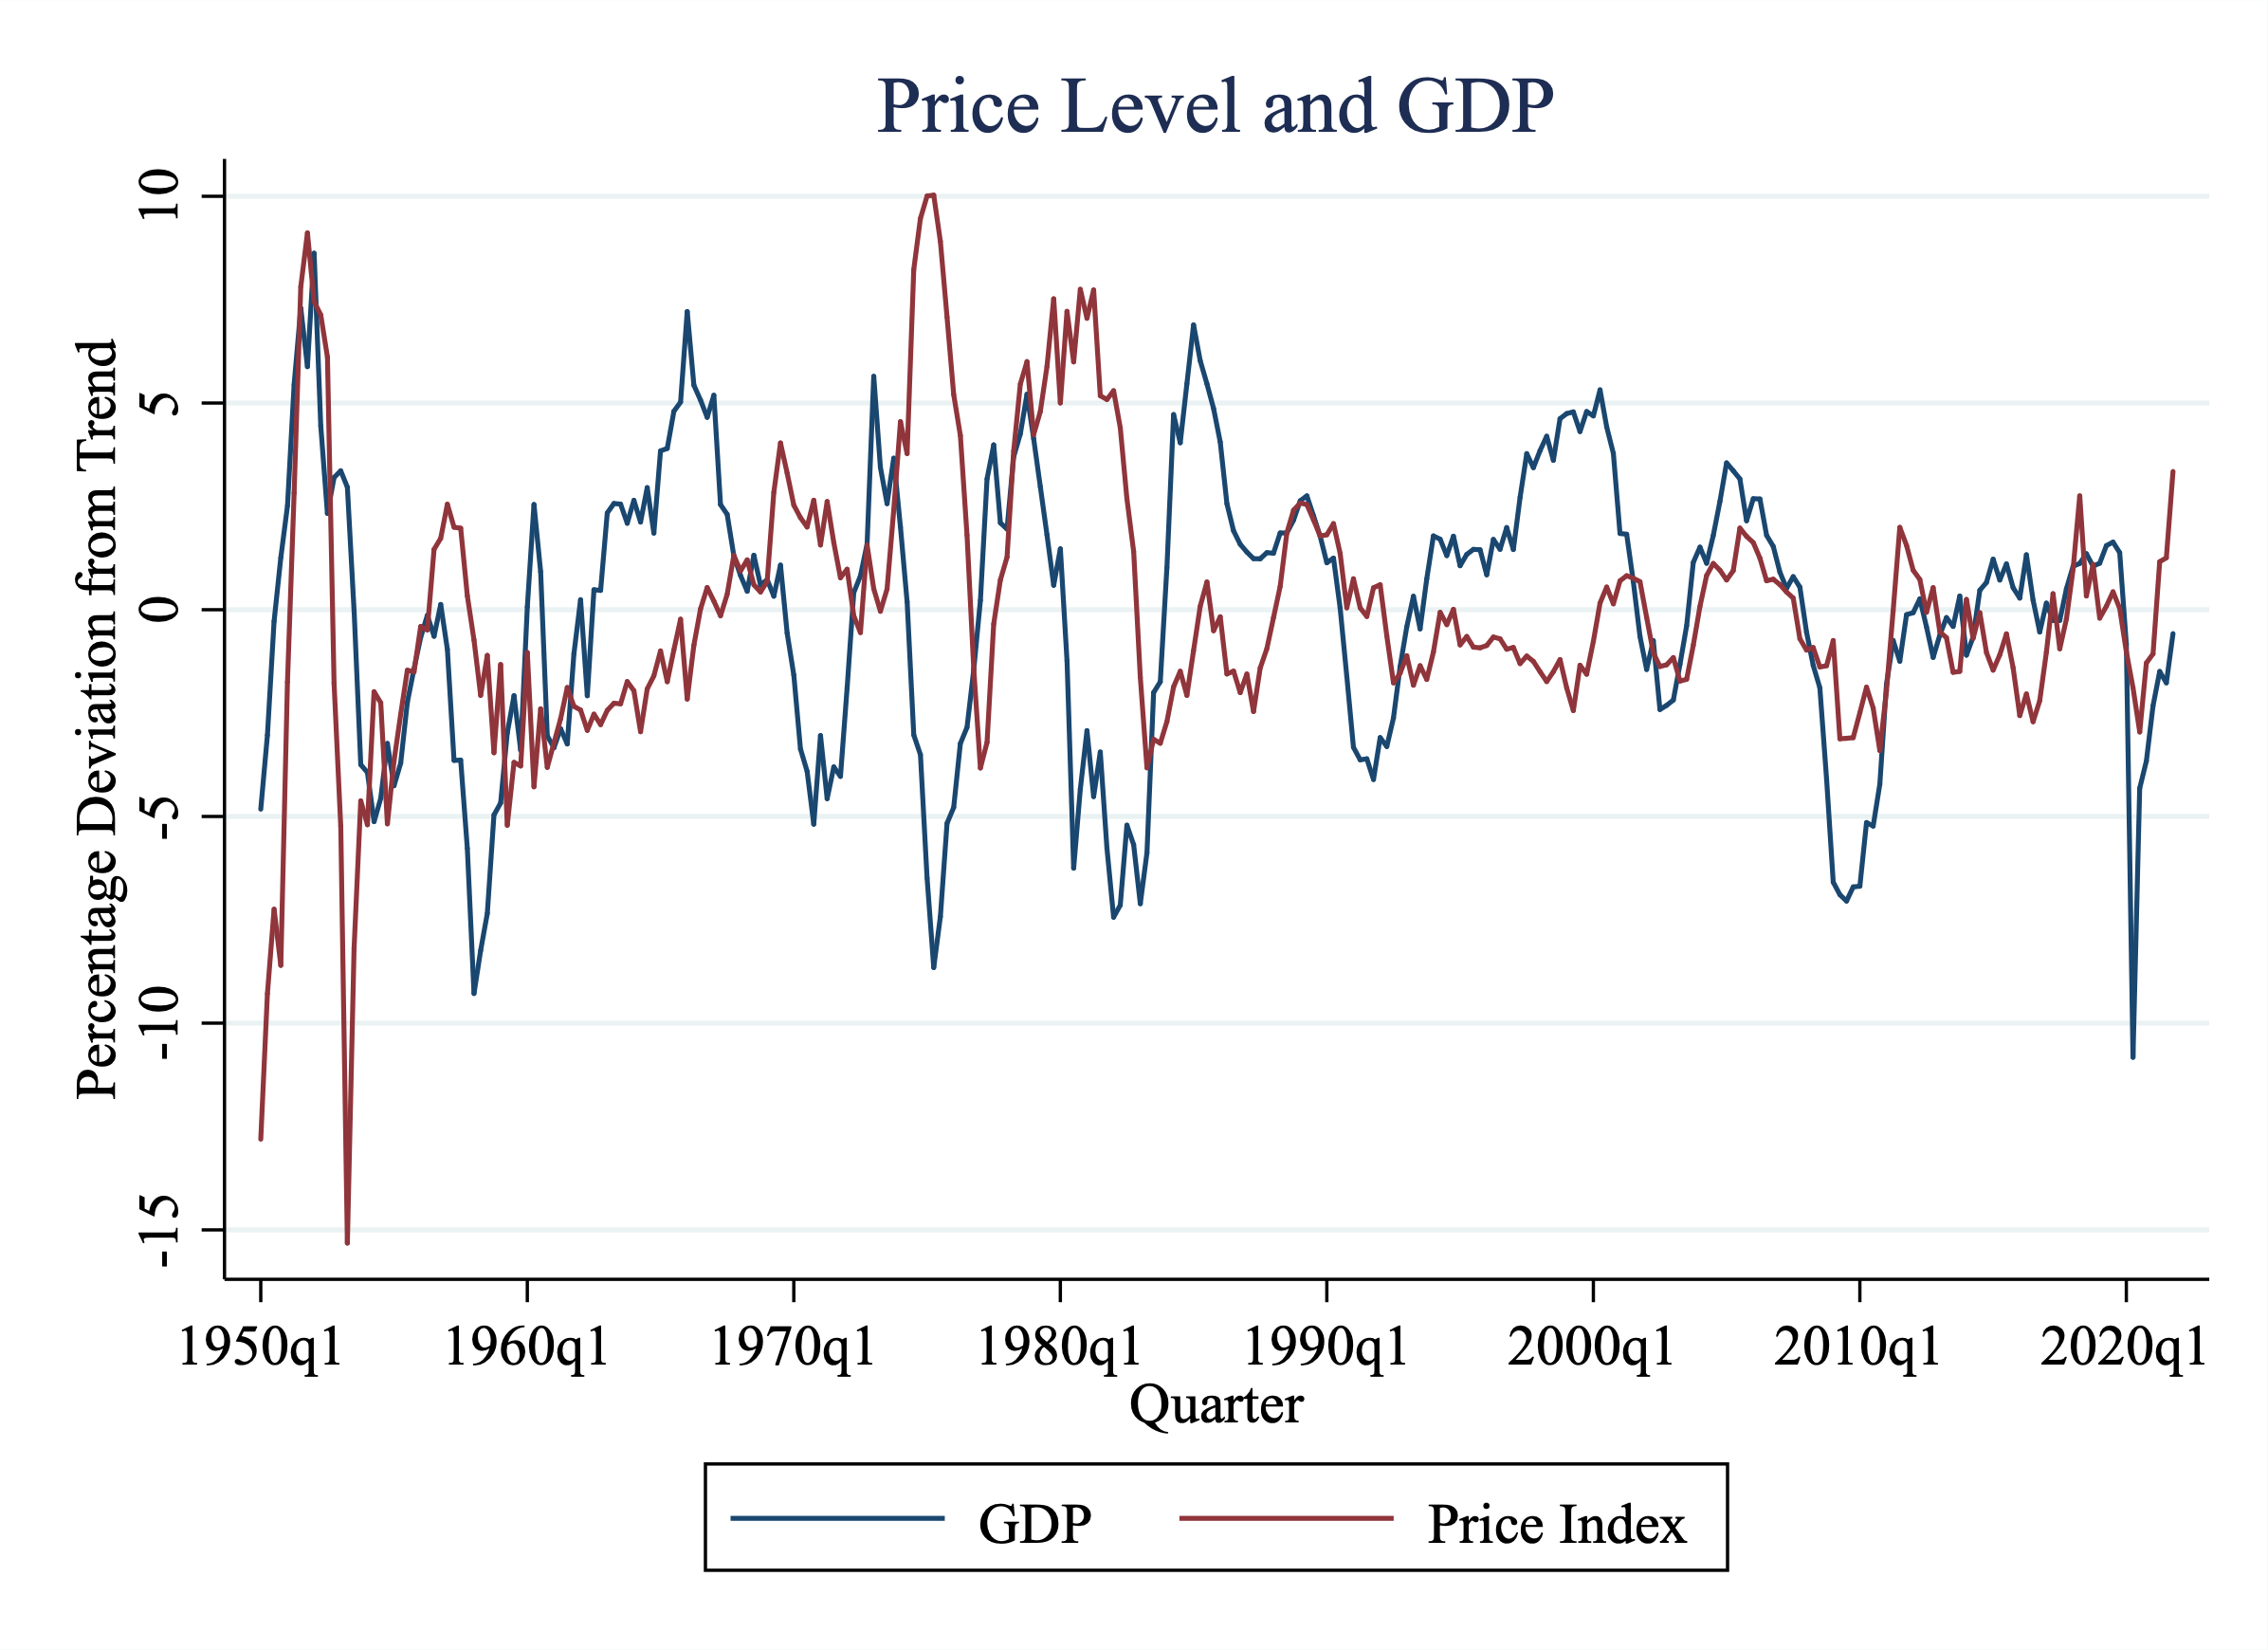
\includegraphics[scale=0.25]{Figures/Fig_3pt11.png}
\end{figure}
\end{frame}


\begin{frame}
\frametitle[alignment=center]{Inflation and Real GDP}
\begin{figure}
\centering
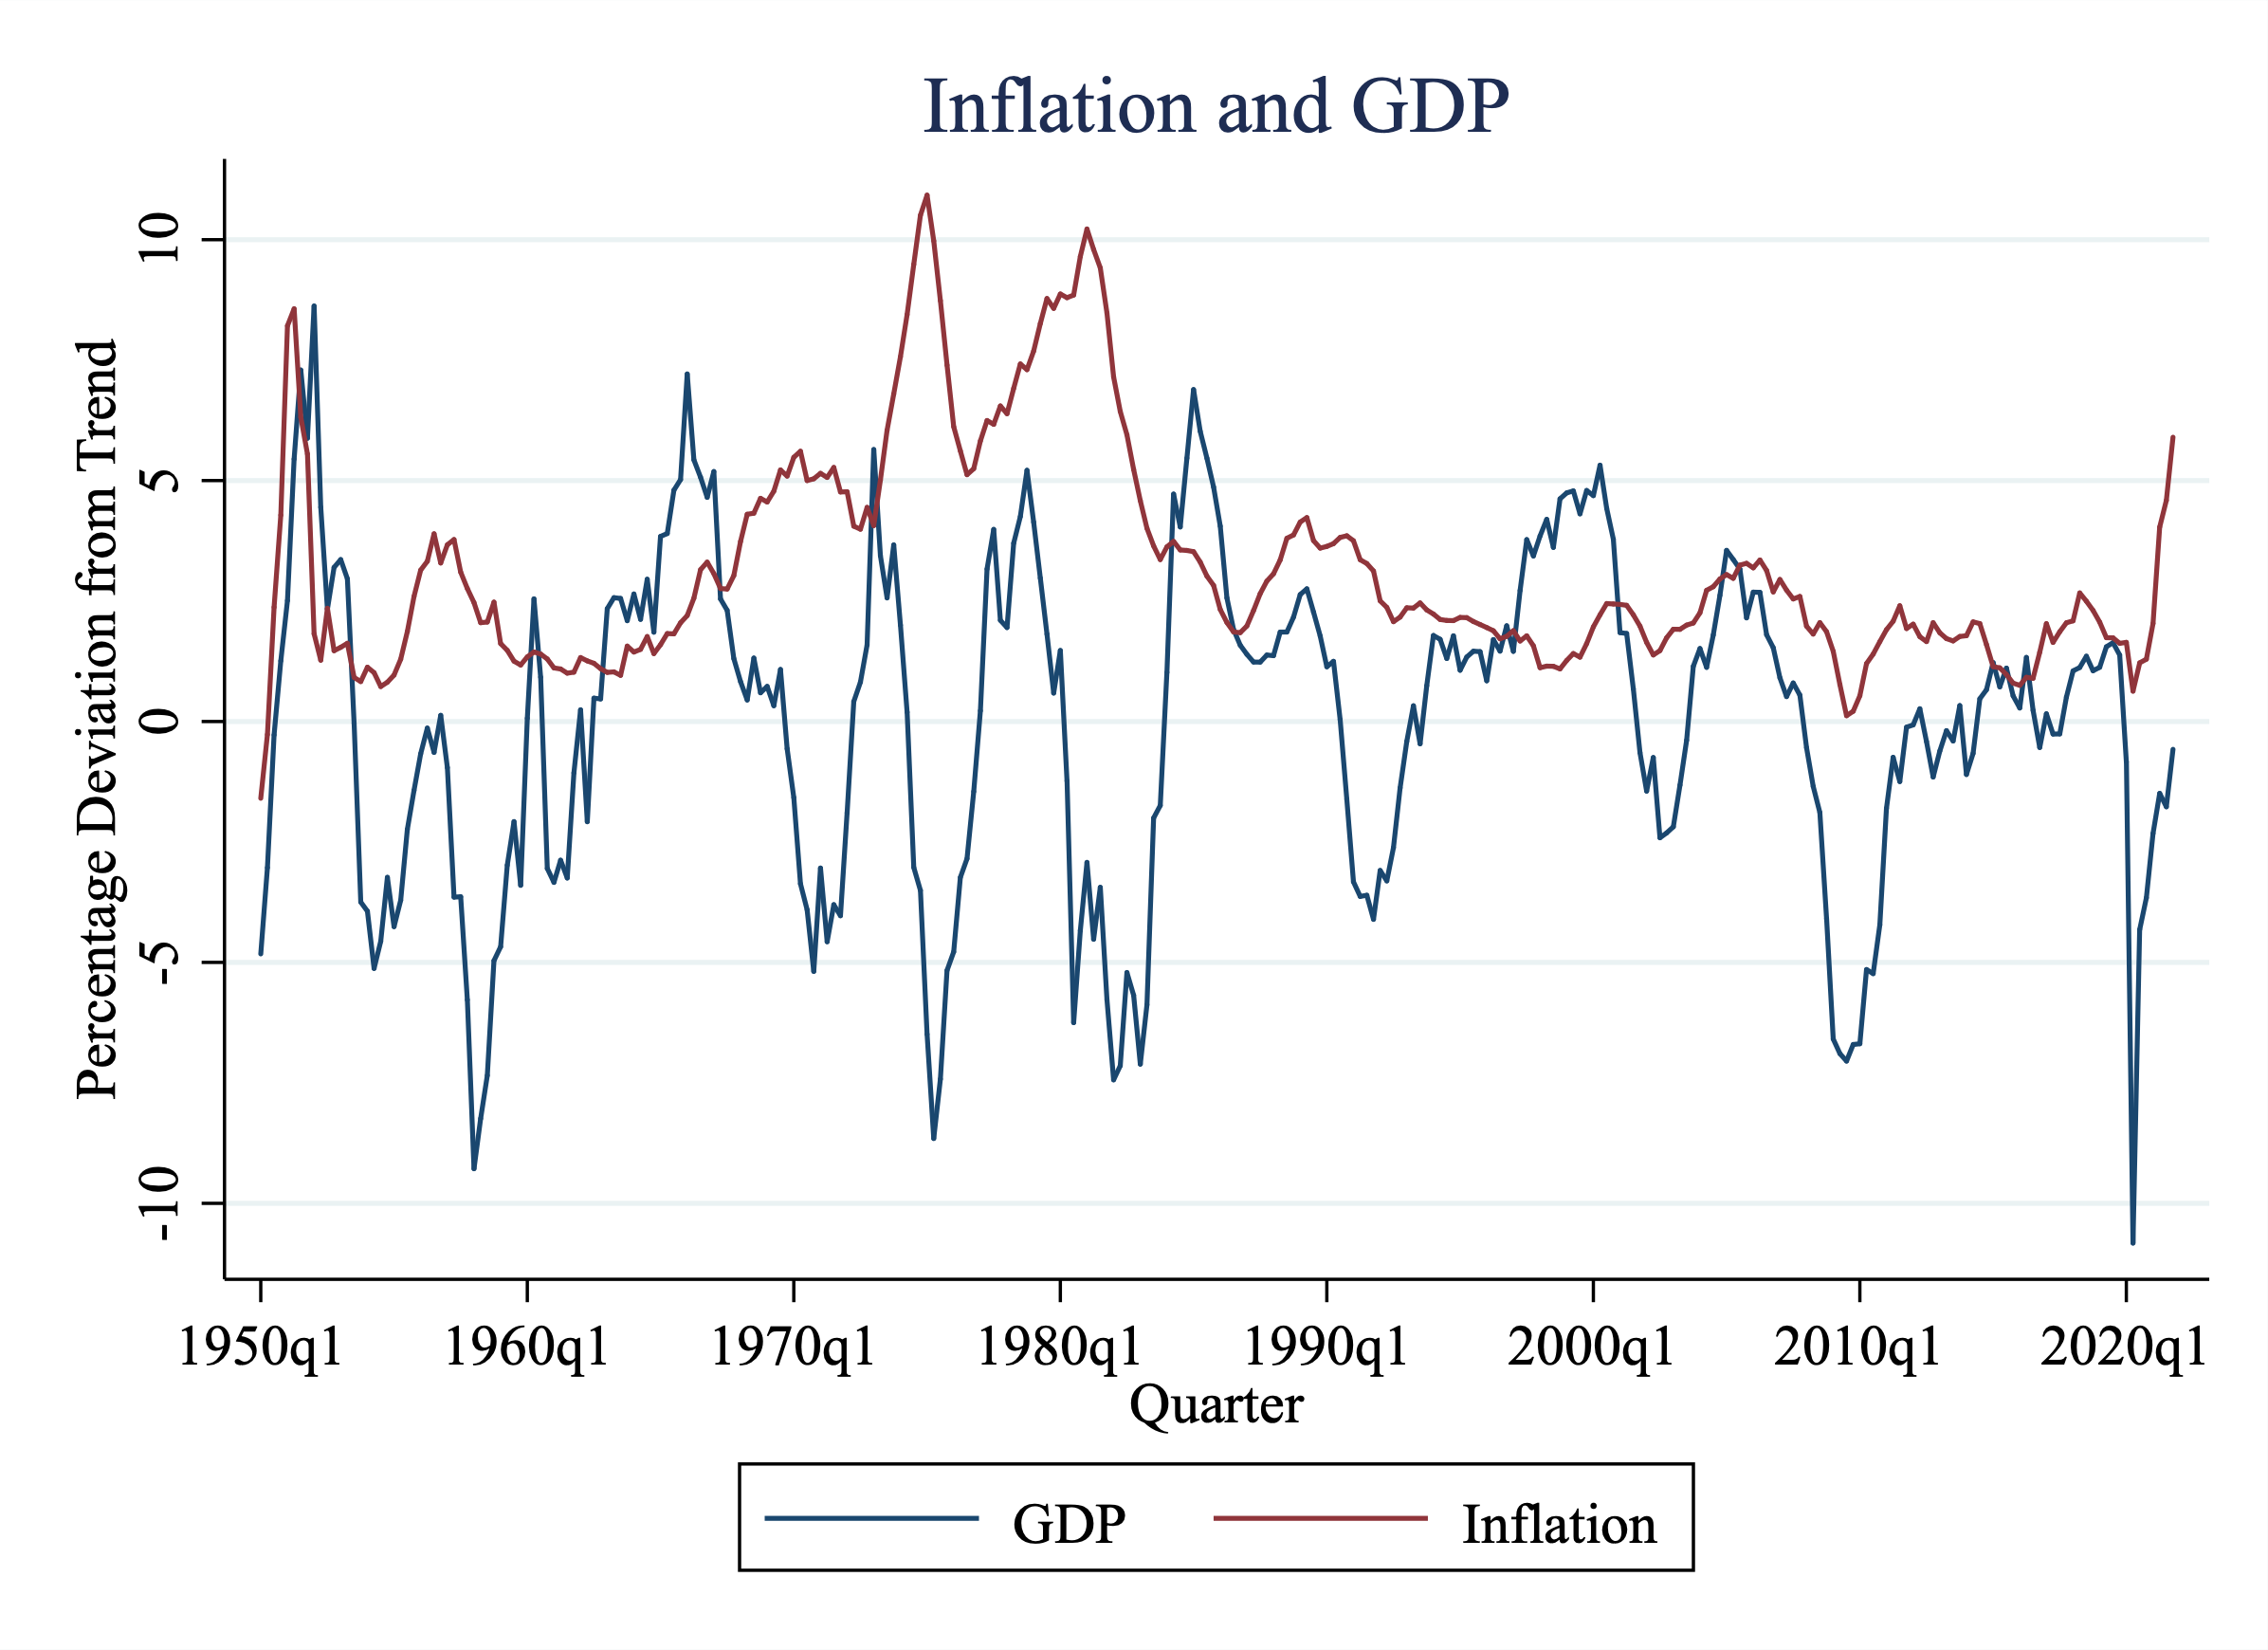
\includegraphics[scale=0.25]{Figures/Fig_3pt12.png}
\end{figure}
\end{frame}

\begin{frame}
\frametitle[alignment=center]{Employment and Real GDP-Williamson}
\begin{figure}
\centering
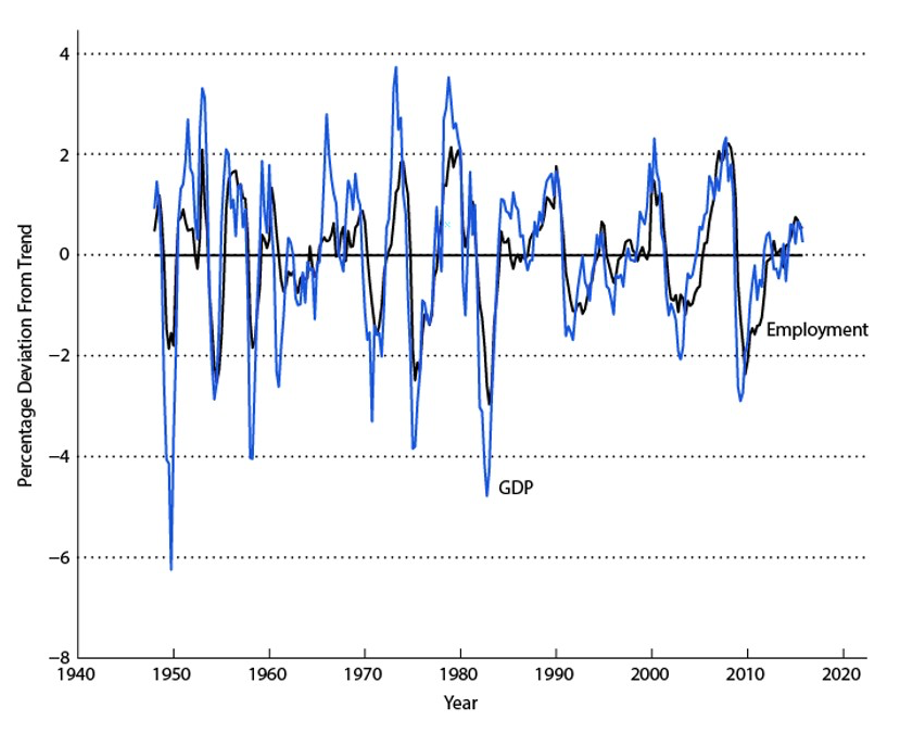
\includegraphics[scale=0.5]{Figures/W_Fig_3pt13.png}
\end{figure}
\end{frame}

\begin{frame}
\frametitle[alignment=center]{Employment and Real GDP - Updated}
\begin{figure}
\centering
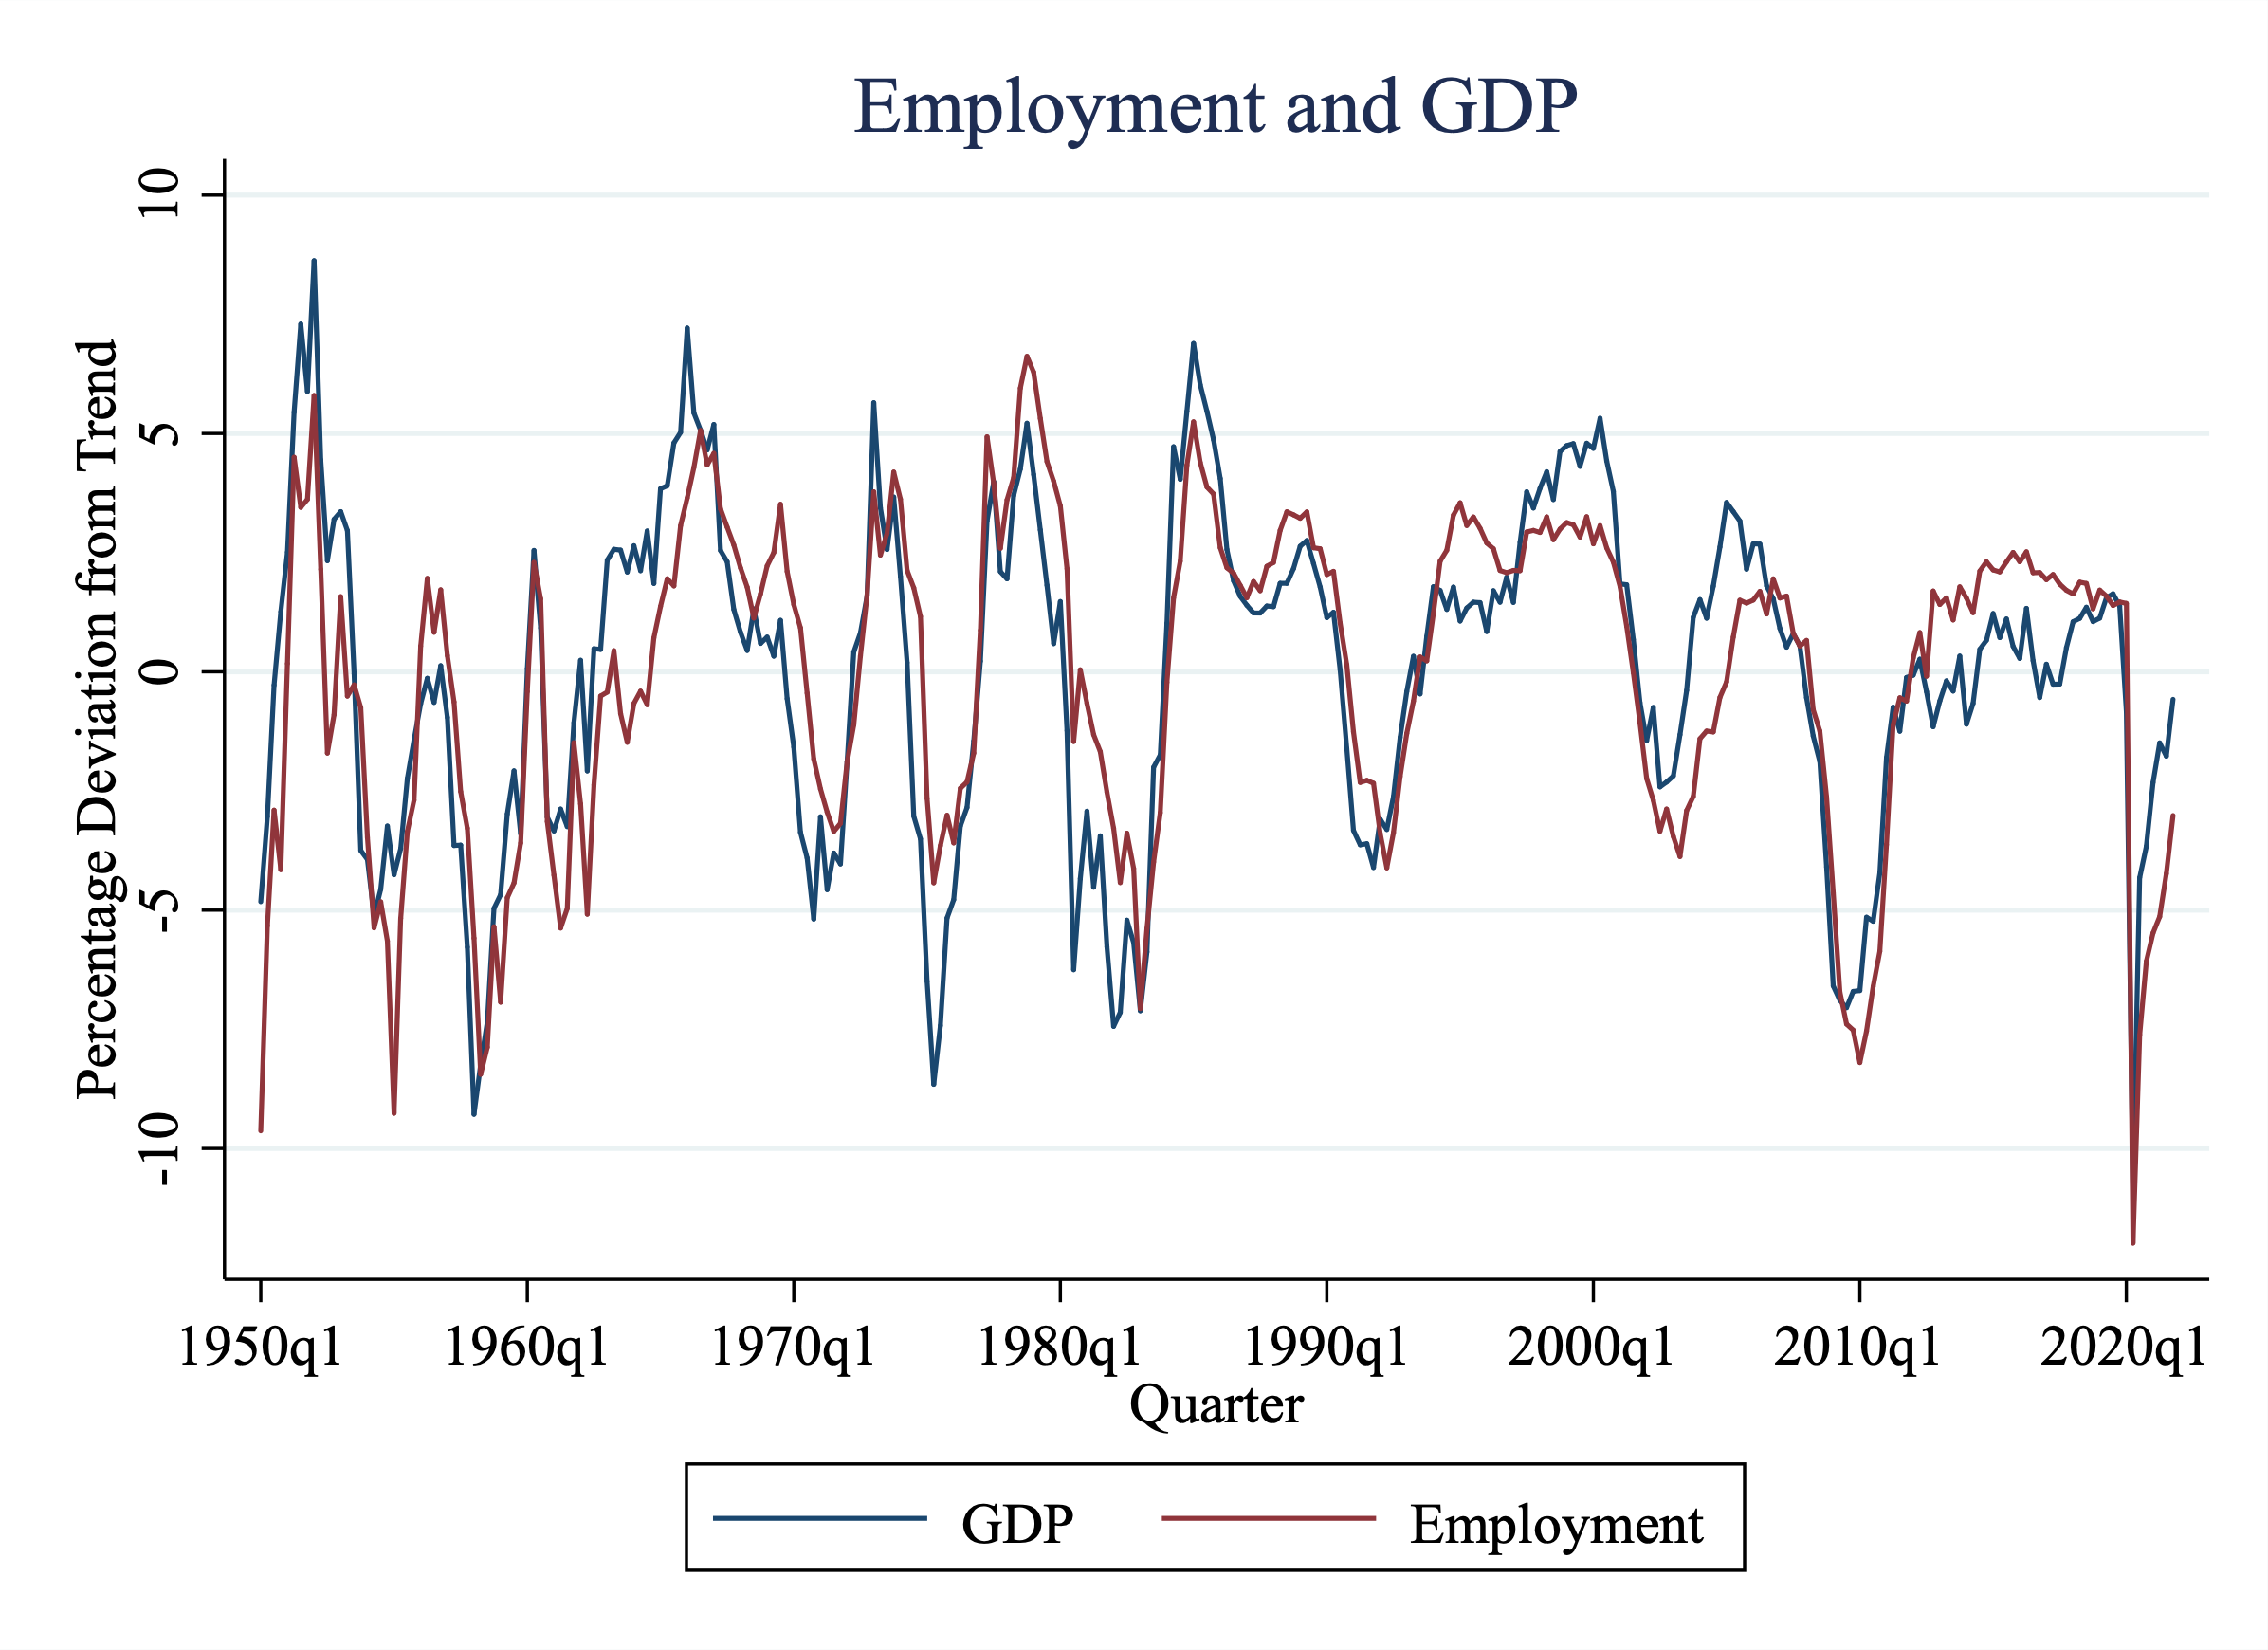
\includegraphics[scale=0.25]{Figures/Fig_3pt13.png}
\end{figure}
\end{frame}





\begin{frame}
\frametitle[alignment=center]{Jobless Recoveries}
\begin{figure}
\centering
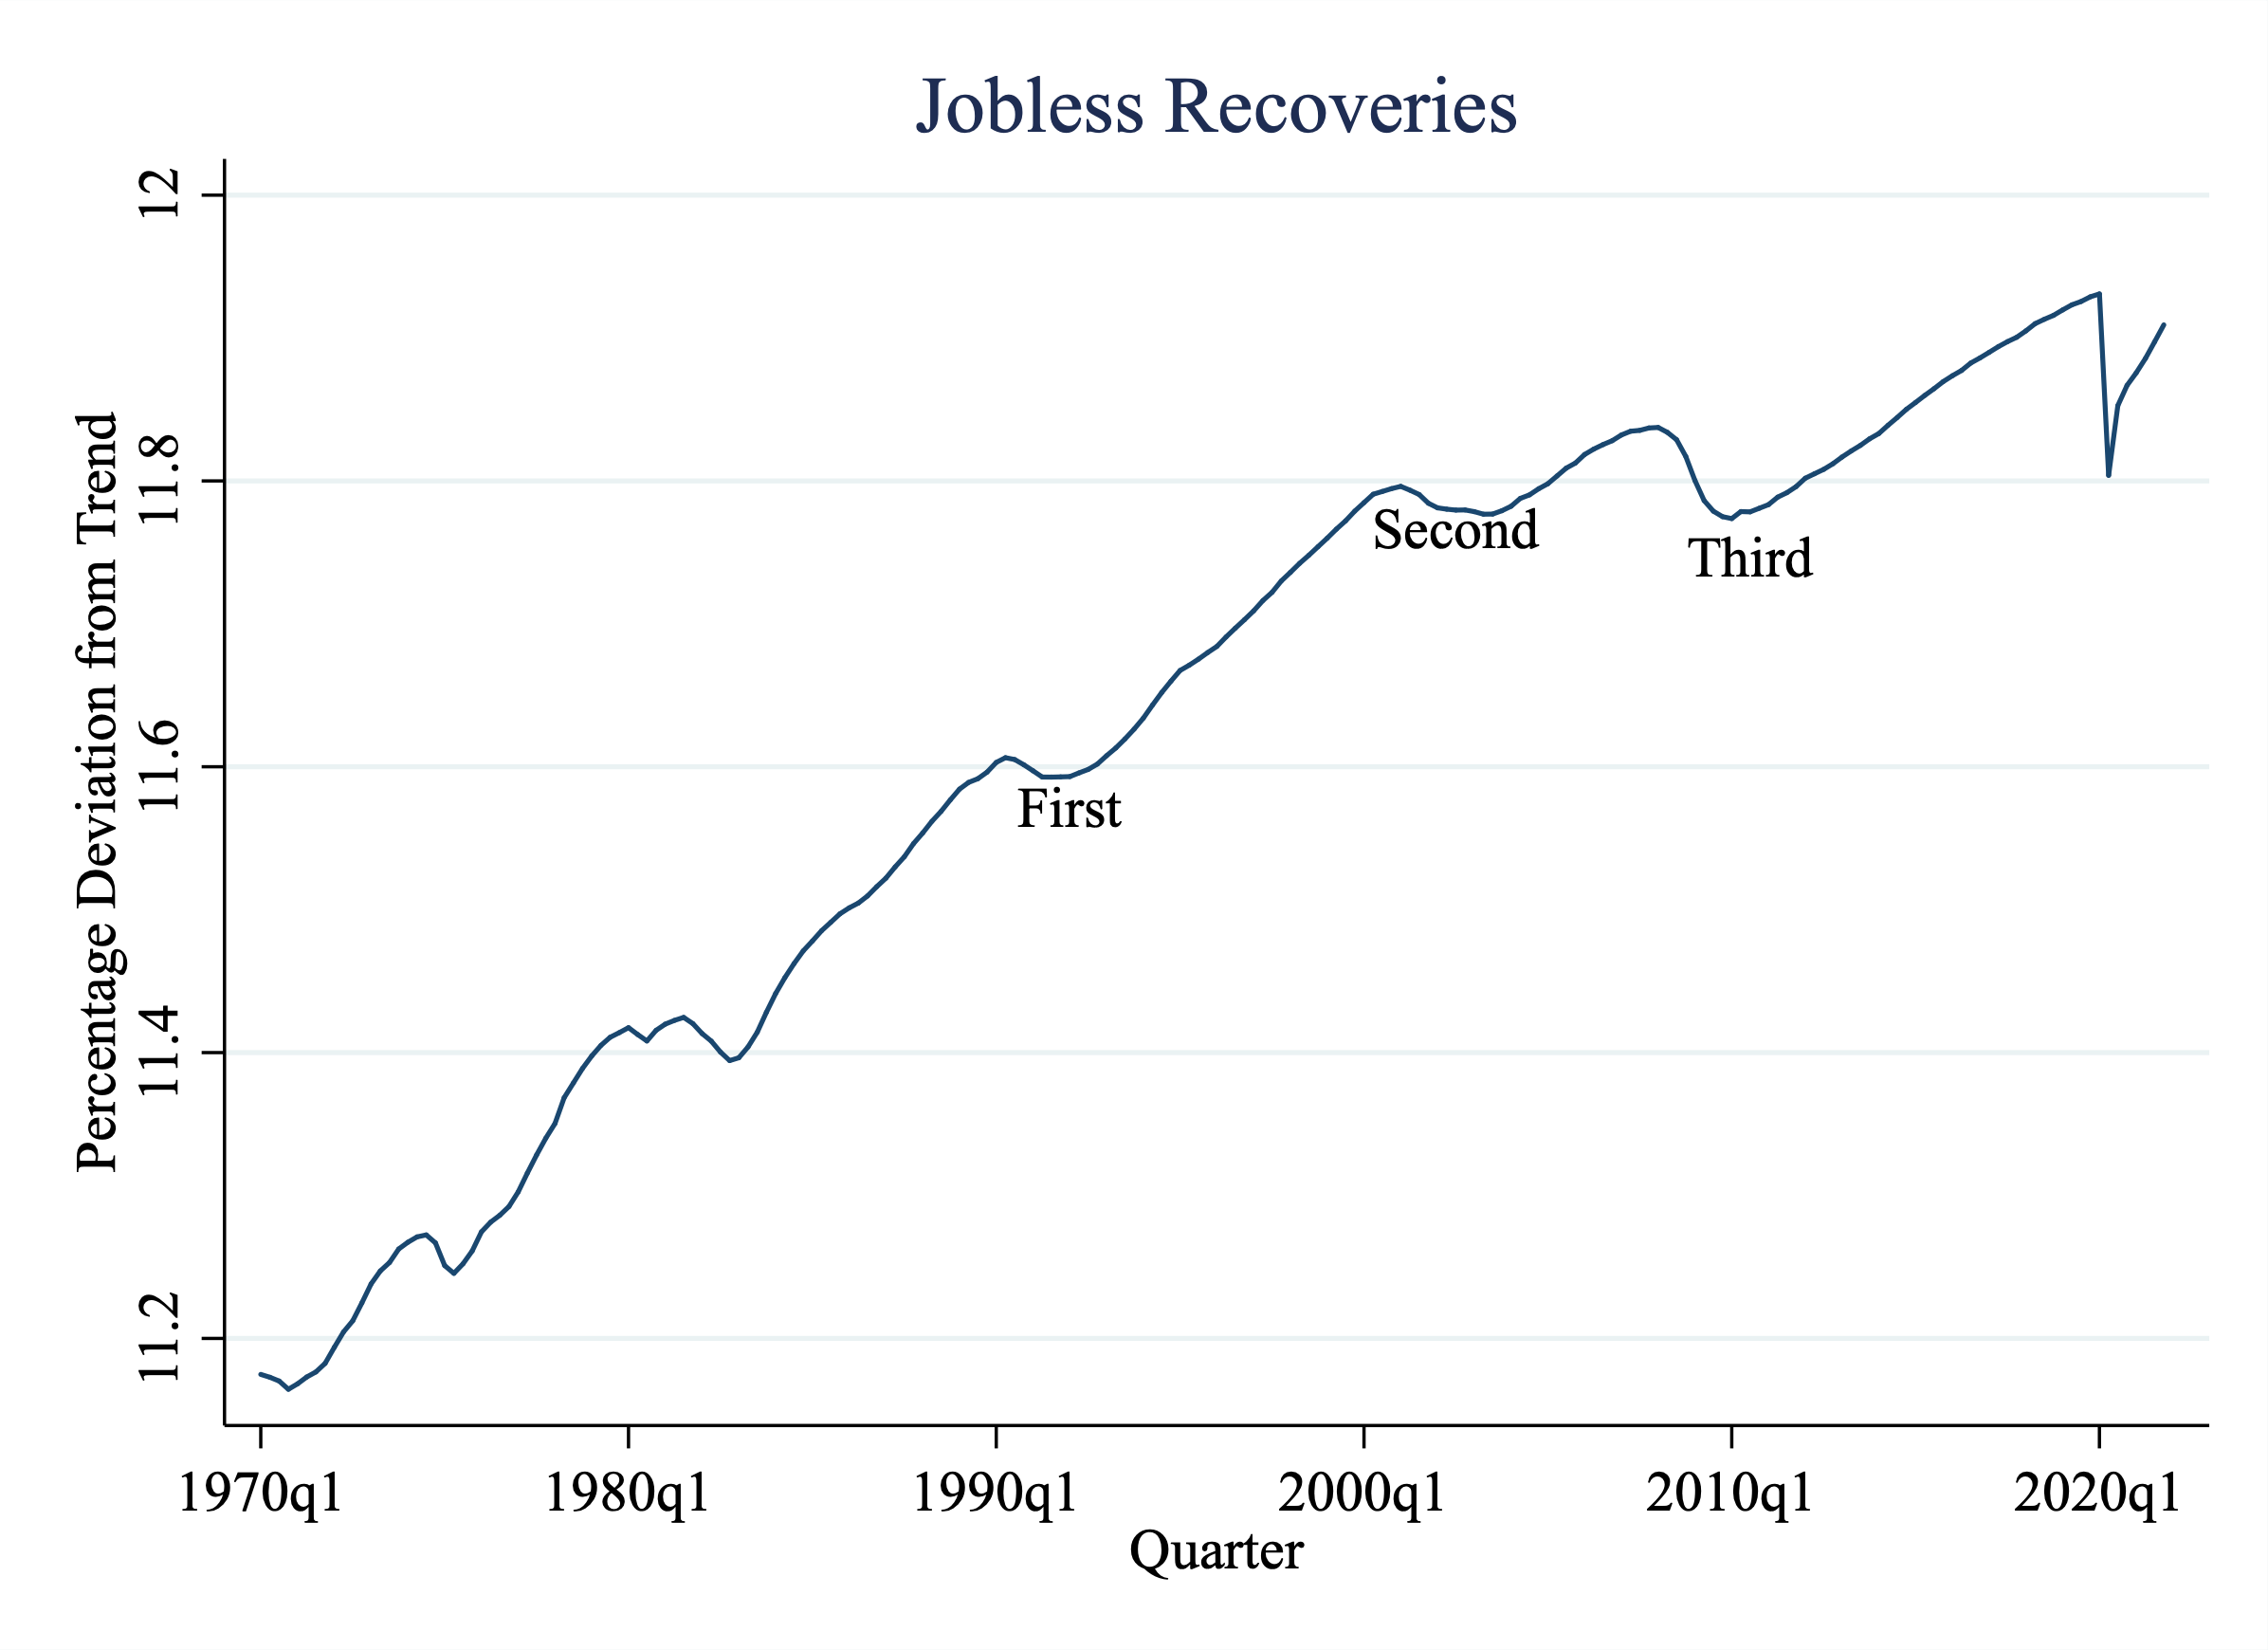
\includegraphics[scale=0.25]{Figures/Fig_3pt14.png}
\end{figure}
\end{frame}

\begin{frame}
\frametitle[alignment=center]{Labor Productivity and Real GDP}
\begin{figure}
\centering
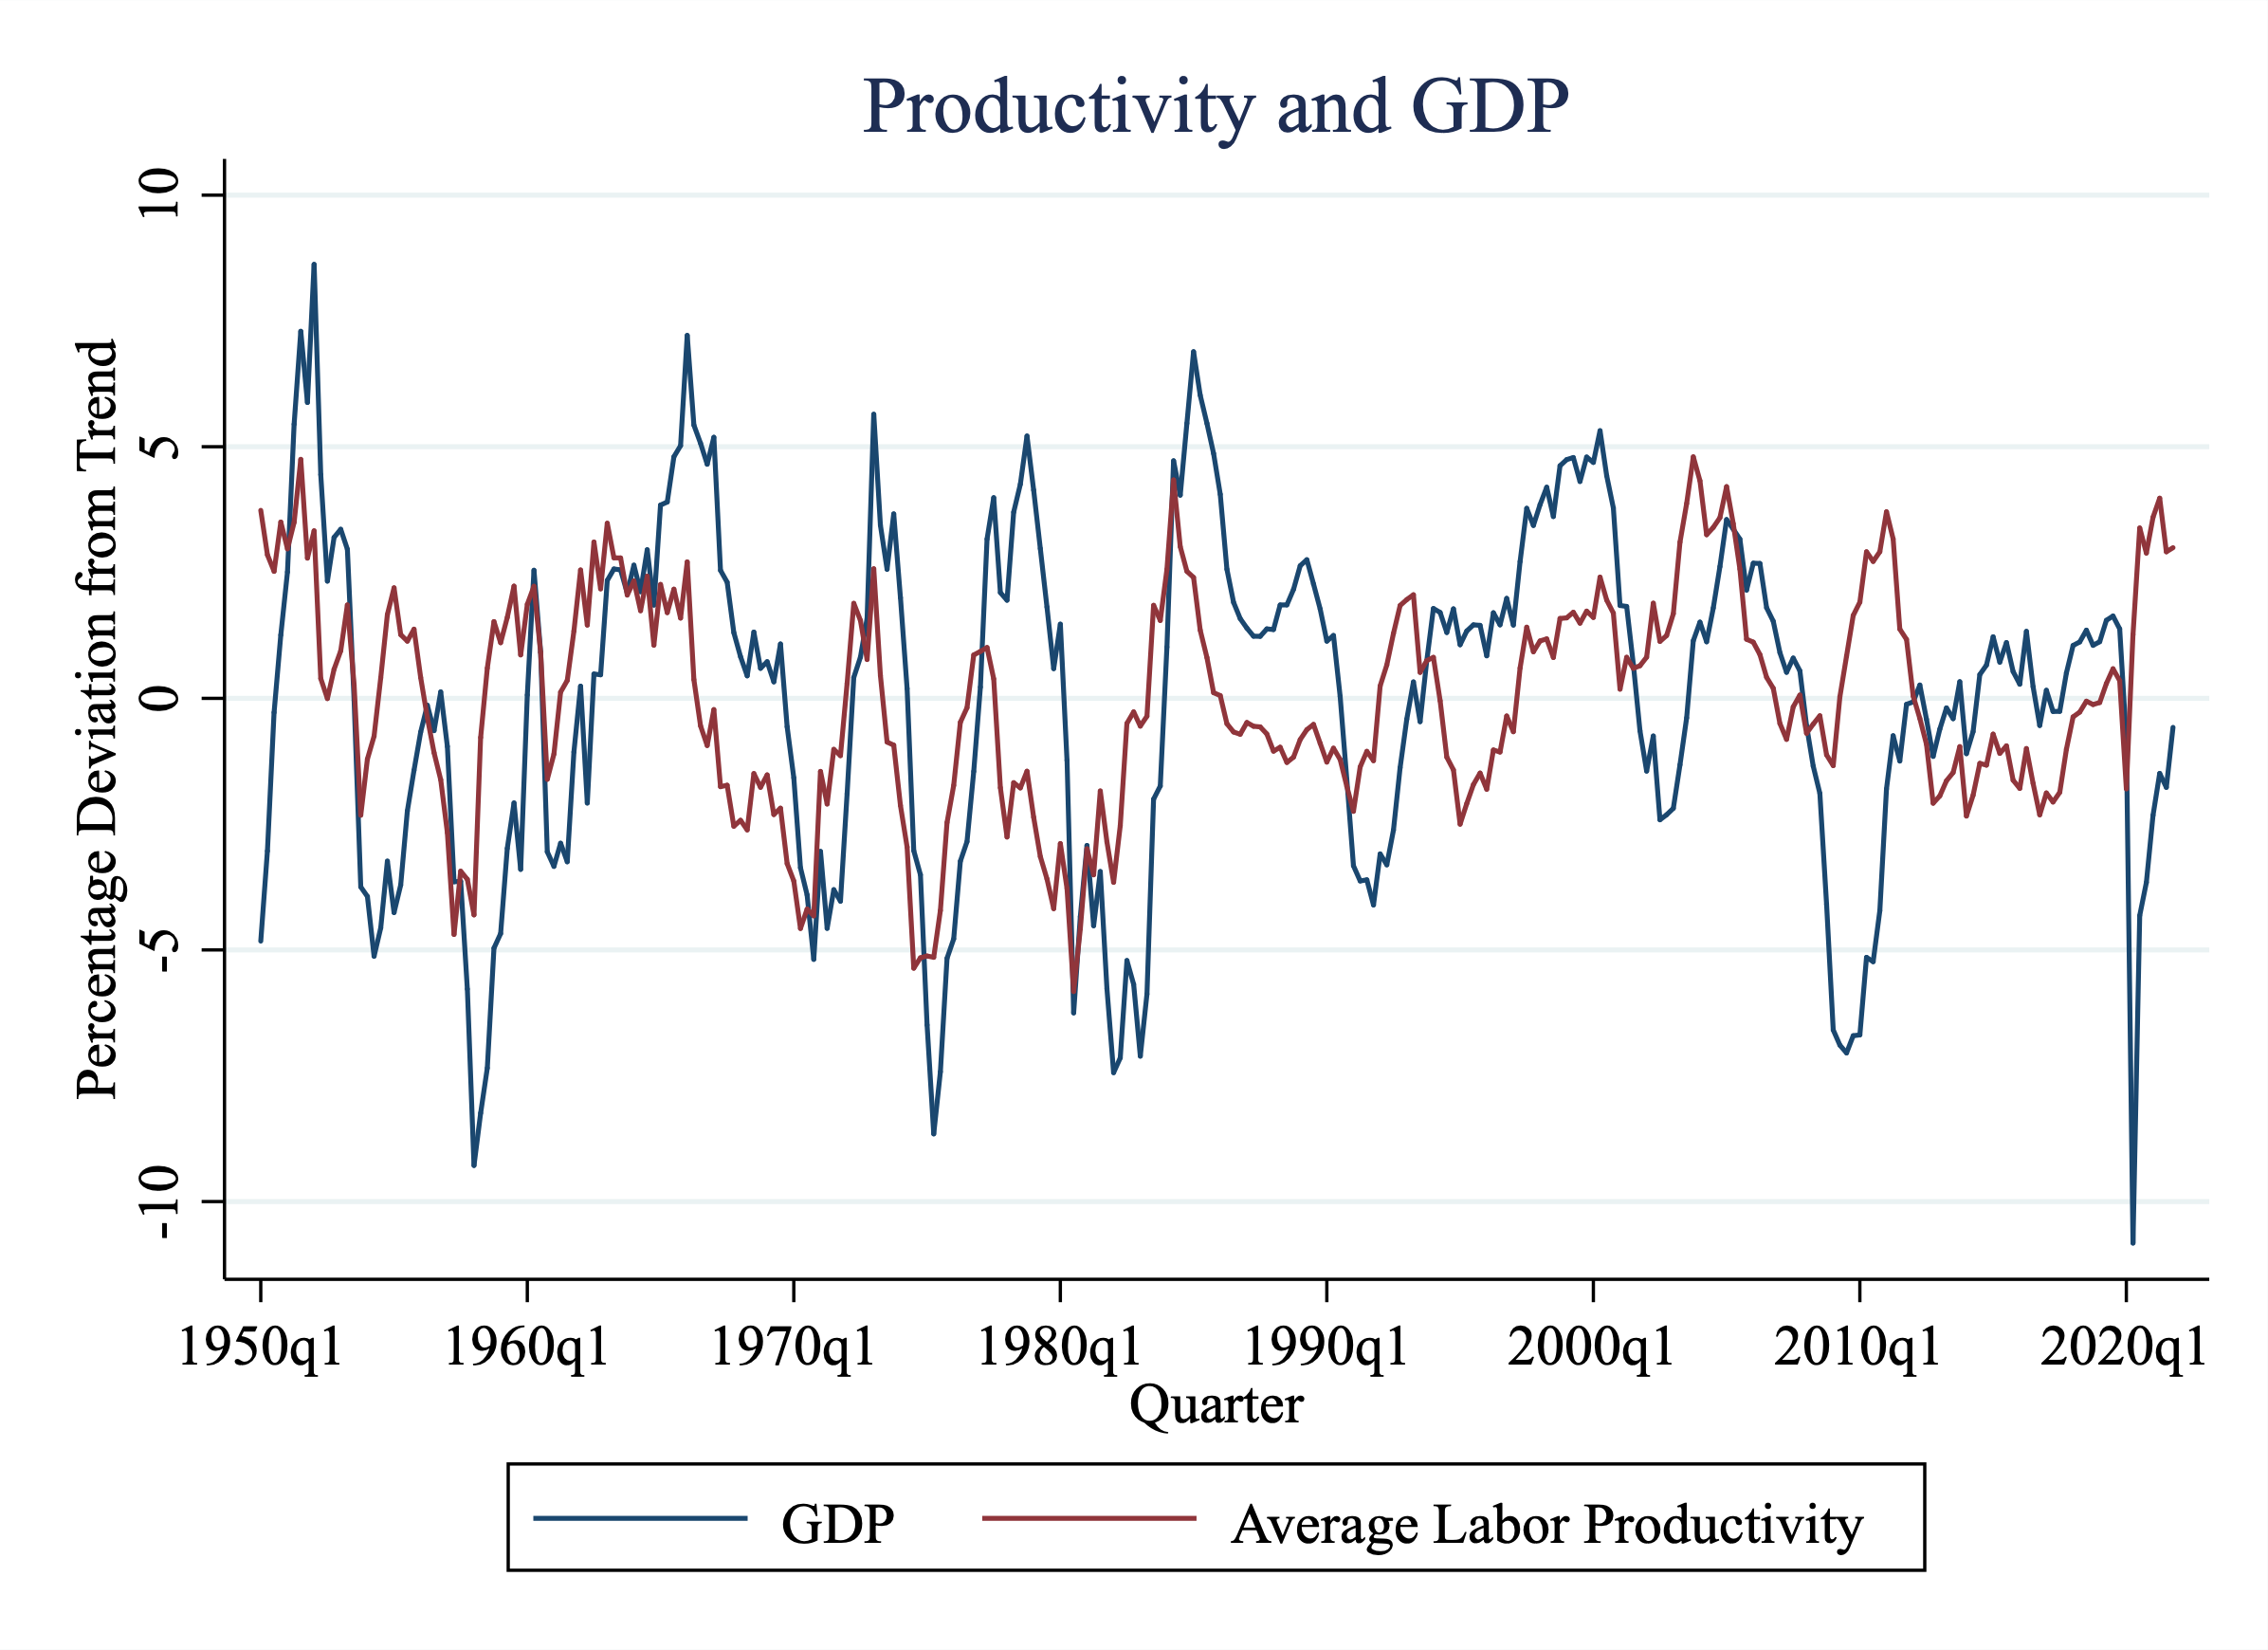
\includegraphics[scale=0.25]{Figures/Fig_3pt15.png}
\end{figure}
\end{frame}

\begin{frame}
\frametitle[alignment=center]{Stock Market and Real GDP}
\begin{figure}
\centering
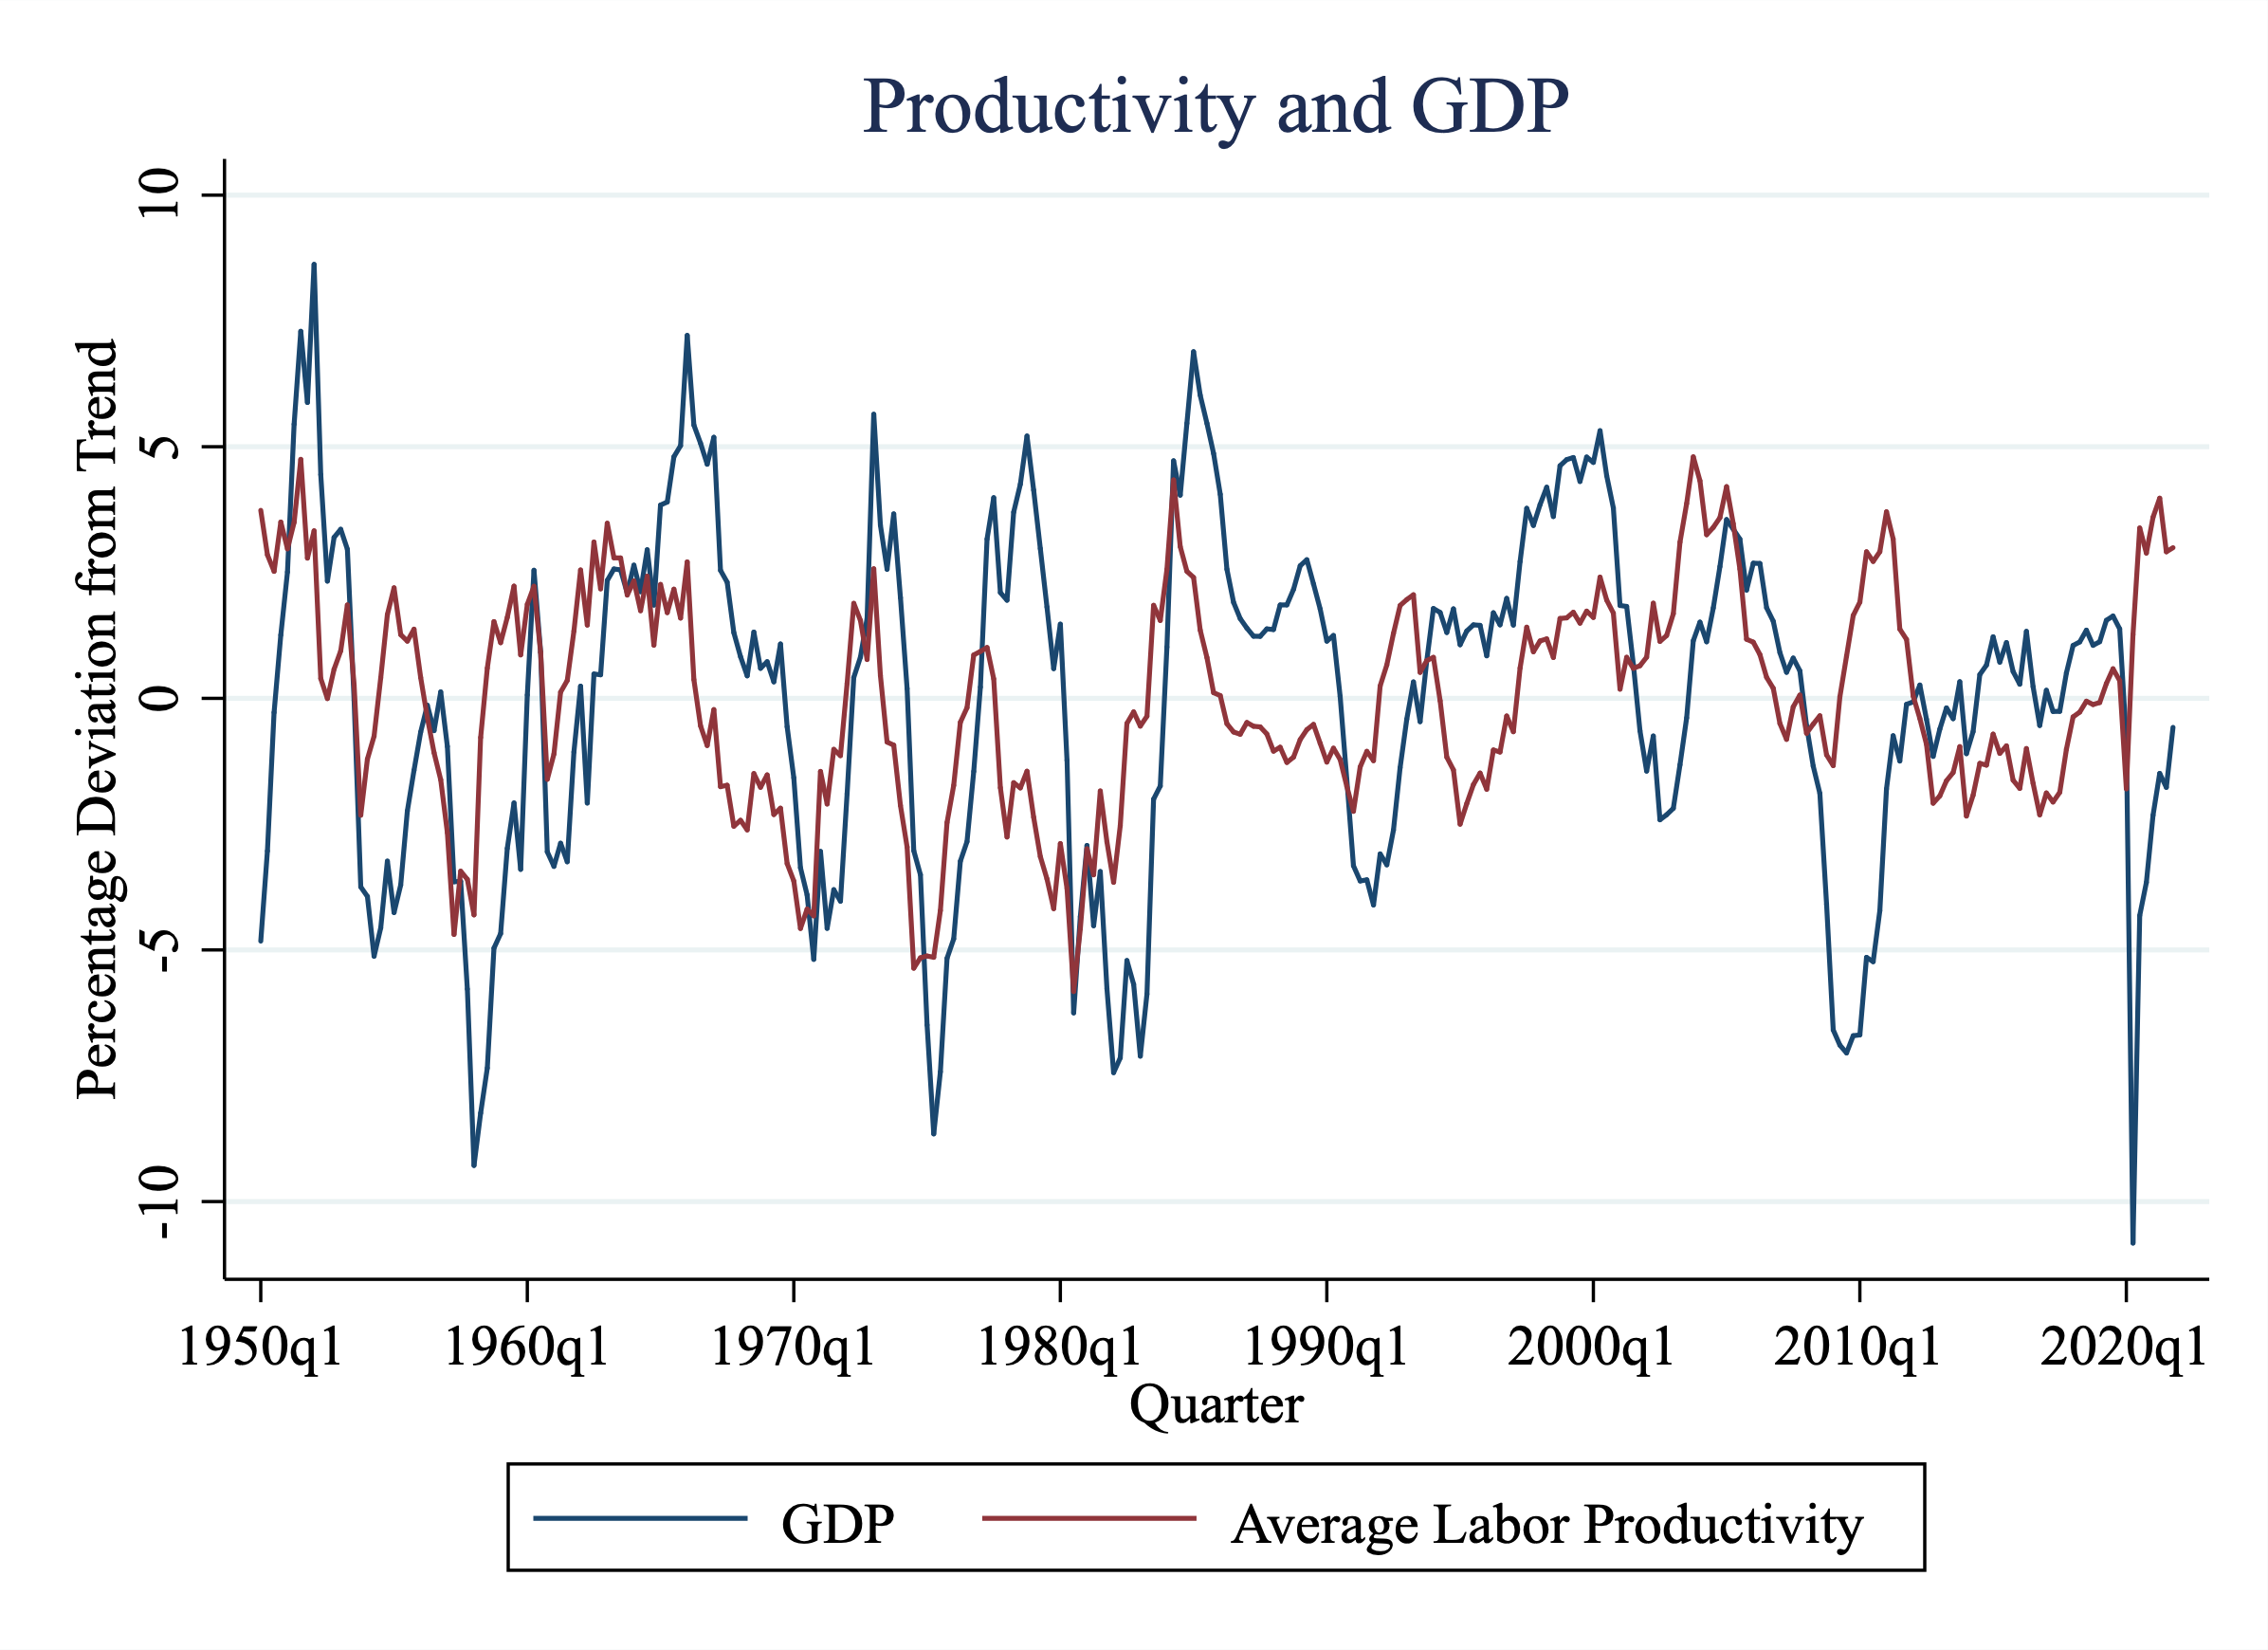
\includegraphics[scale=0.25]{Figures/Fig_3pt15.png}
\end{figure}
\end{frame}


\begin{frame}
\frametitle[alignment=center]{Seasonally Adjusted and Unadjusted Unemployment}
\begin{figure}
\centering
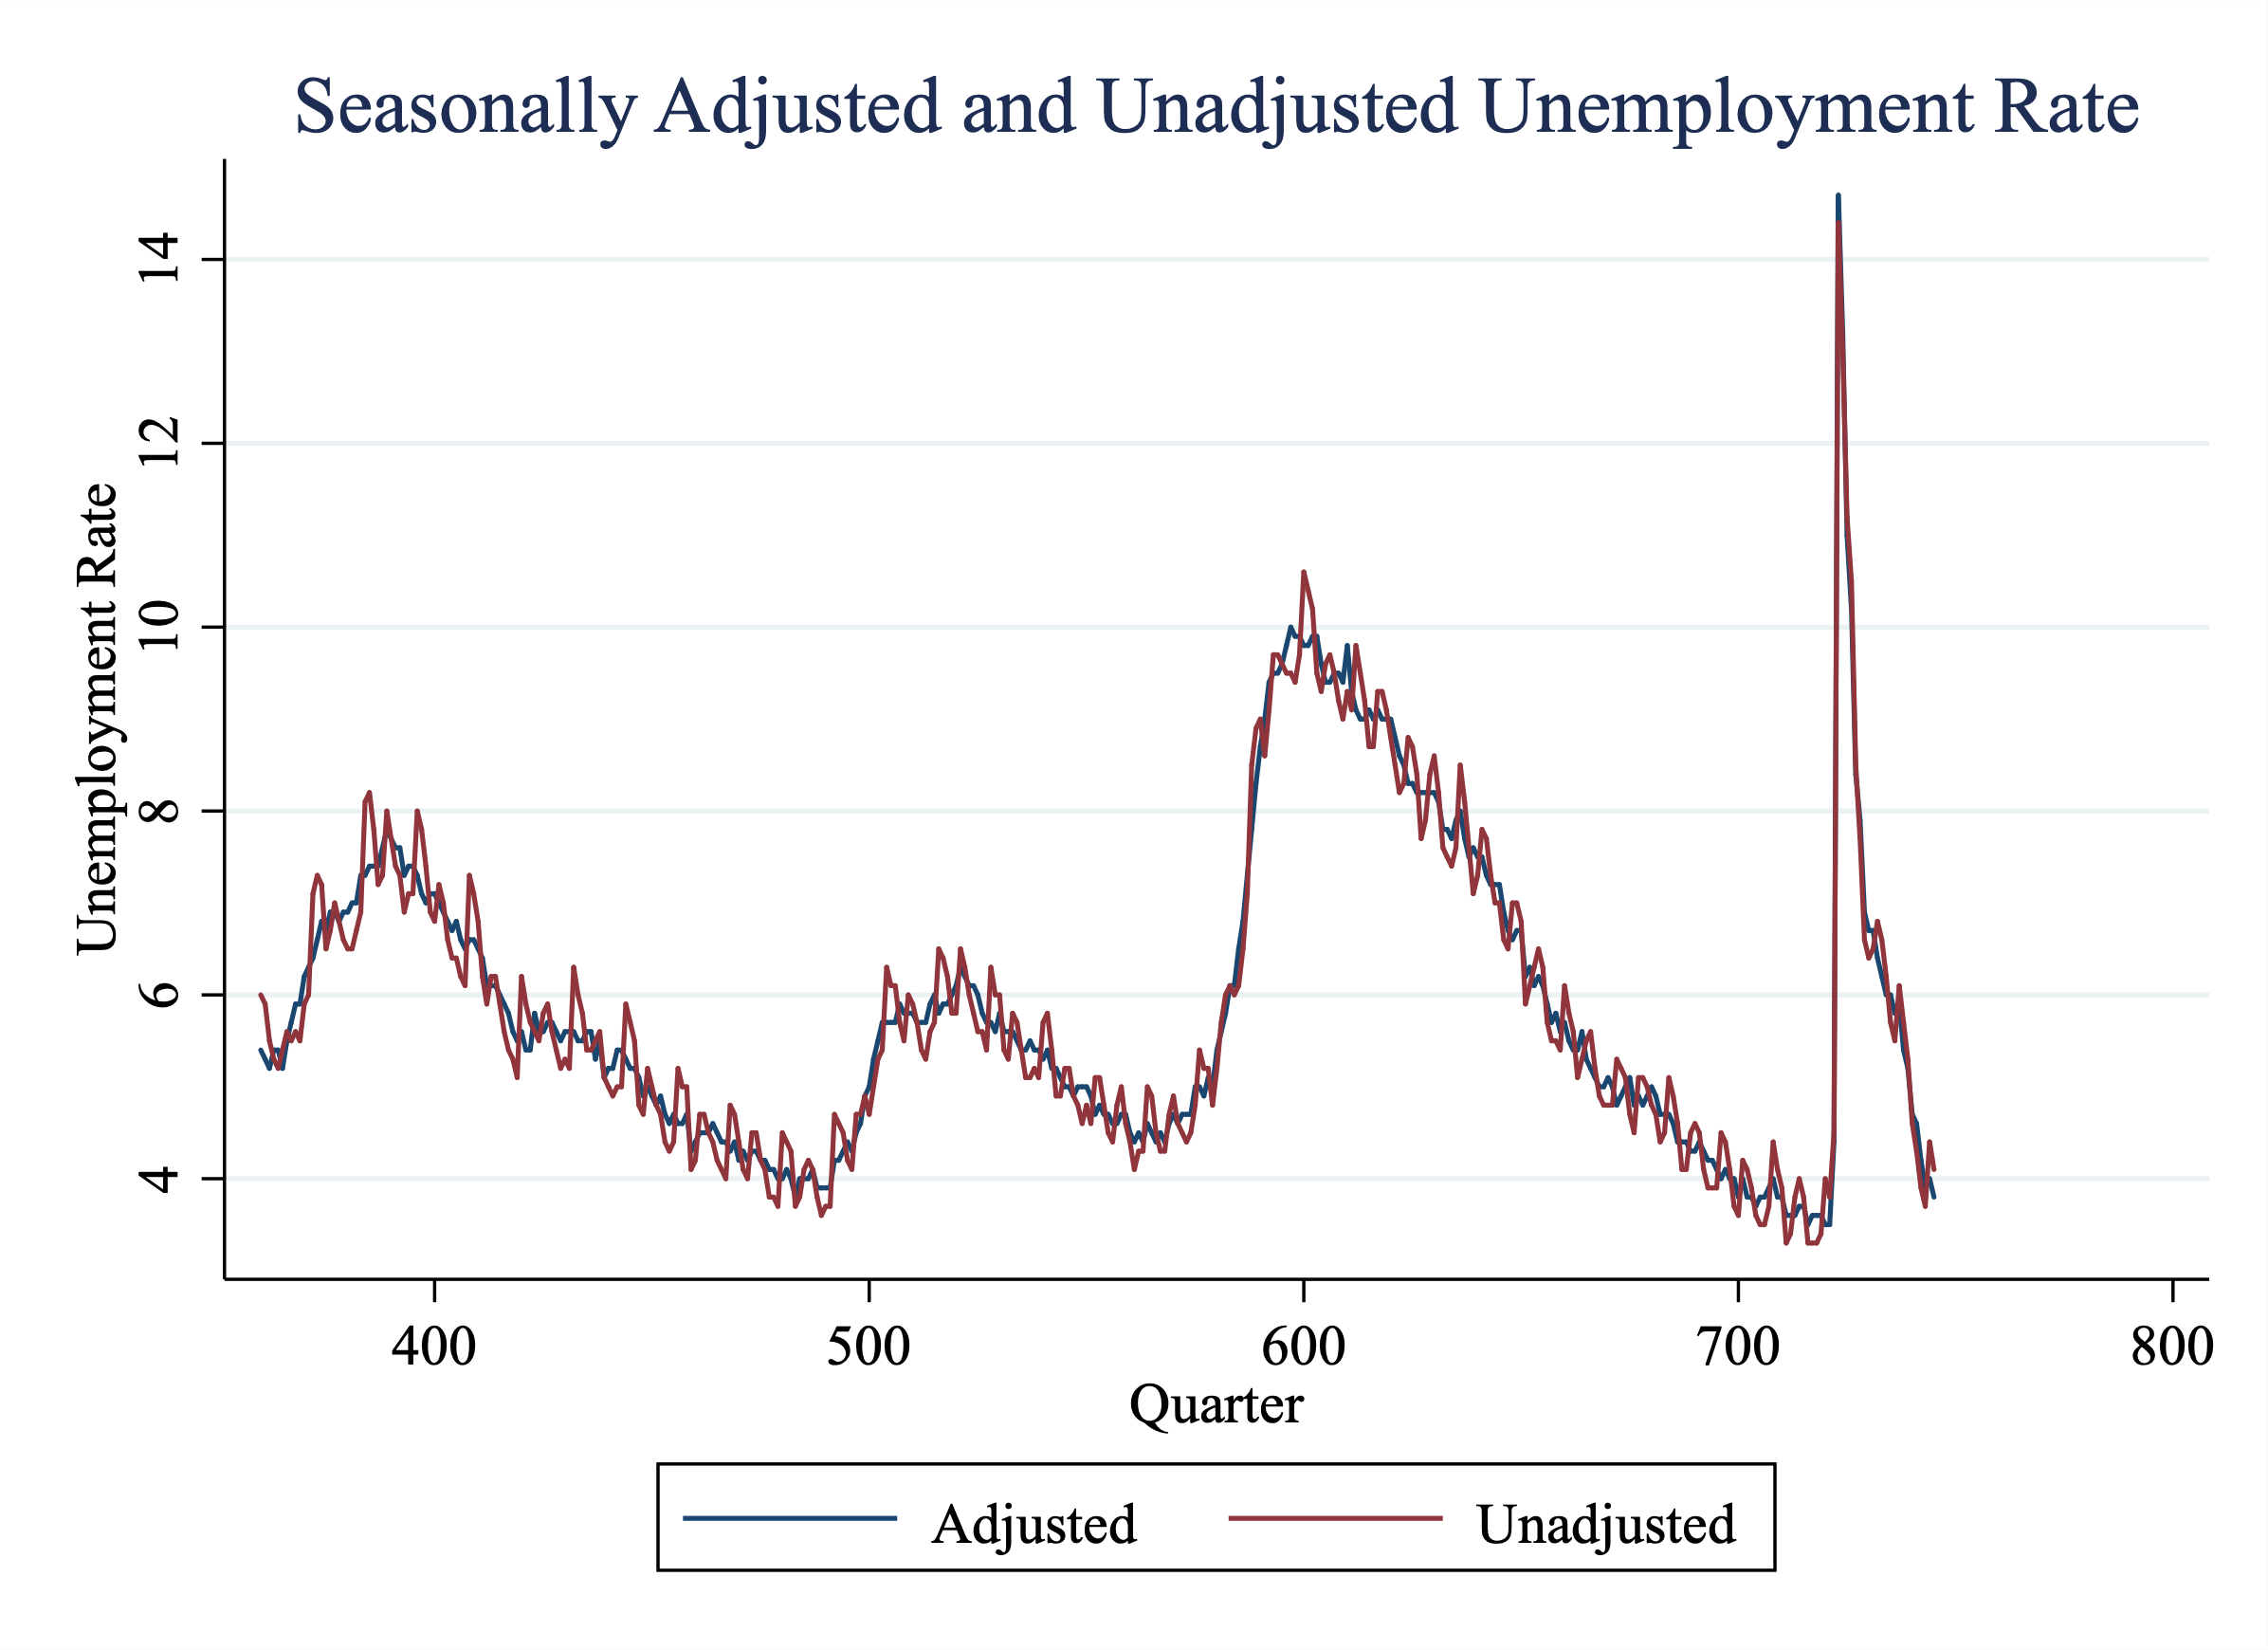
\includegraphics[scale=0.25]{Figures/Fig_3pt16.png}
\end{figure}
\end{frame}

\begin{frame}
\frametitle[alignment=center]{Seasonally Adjusted and Unadjusted Unemployment}
\begin{figure}
\centering
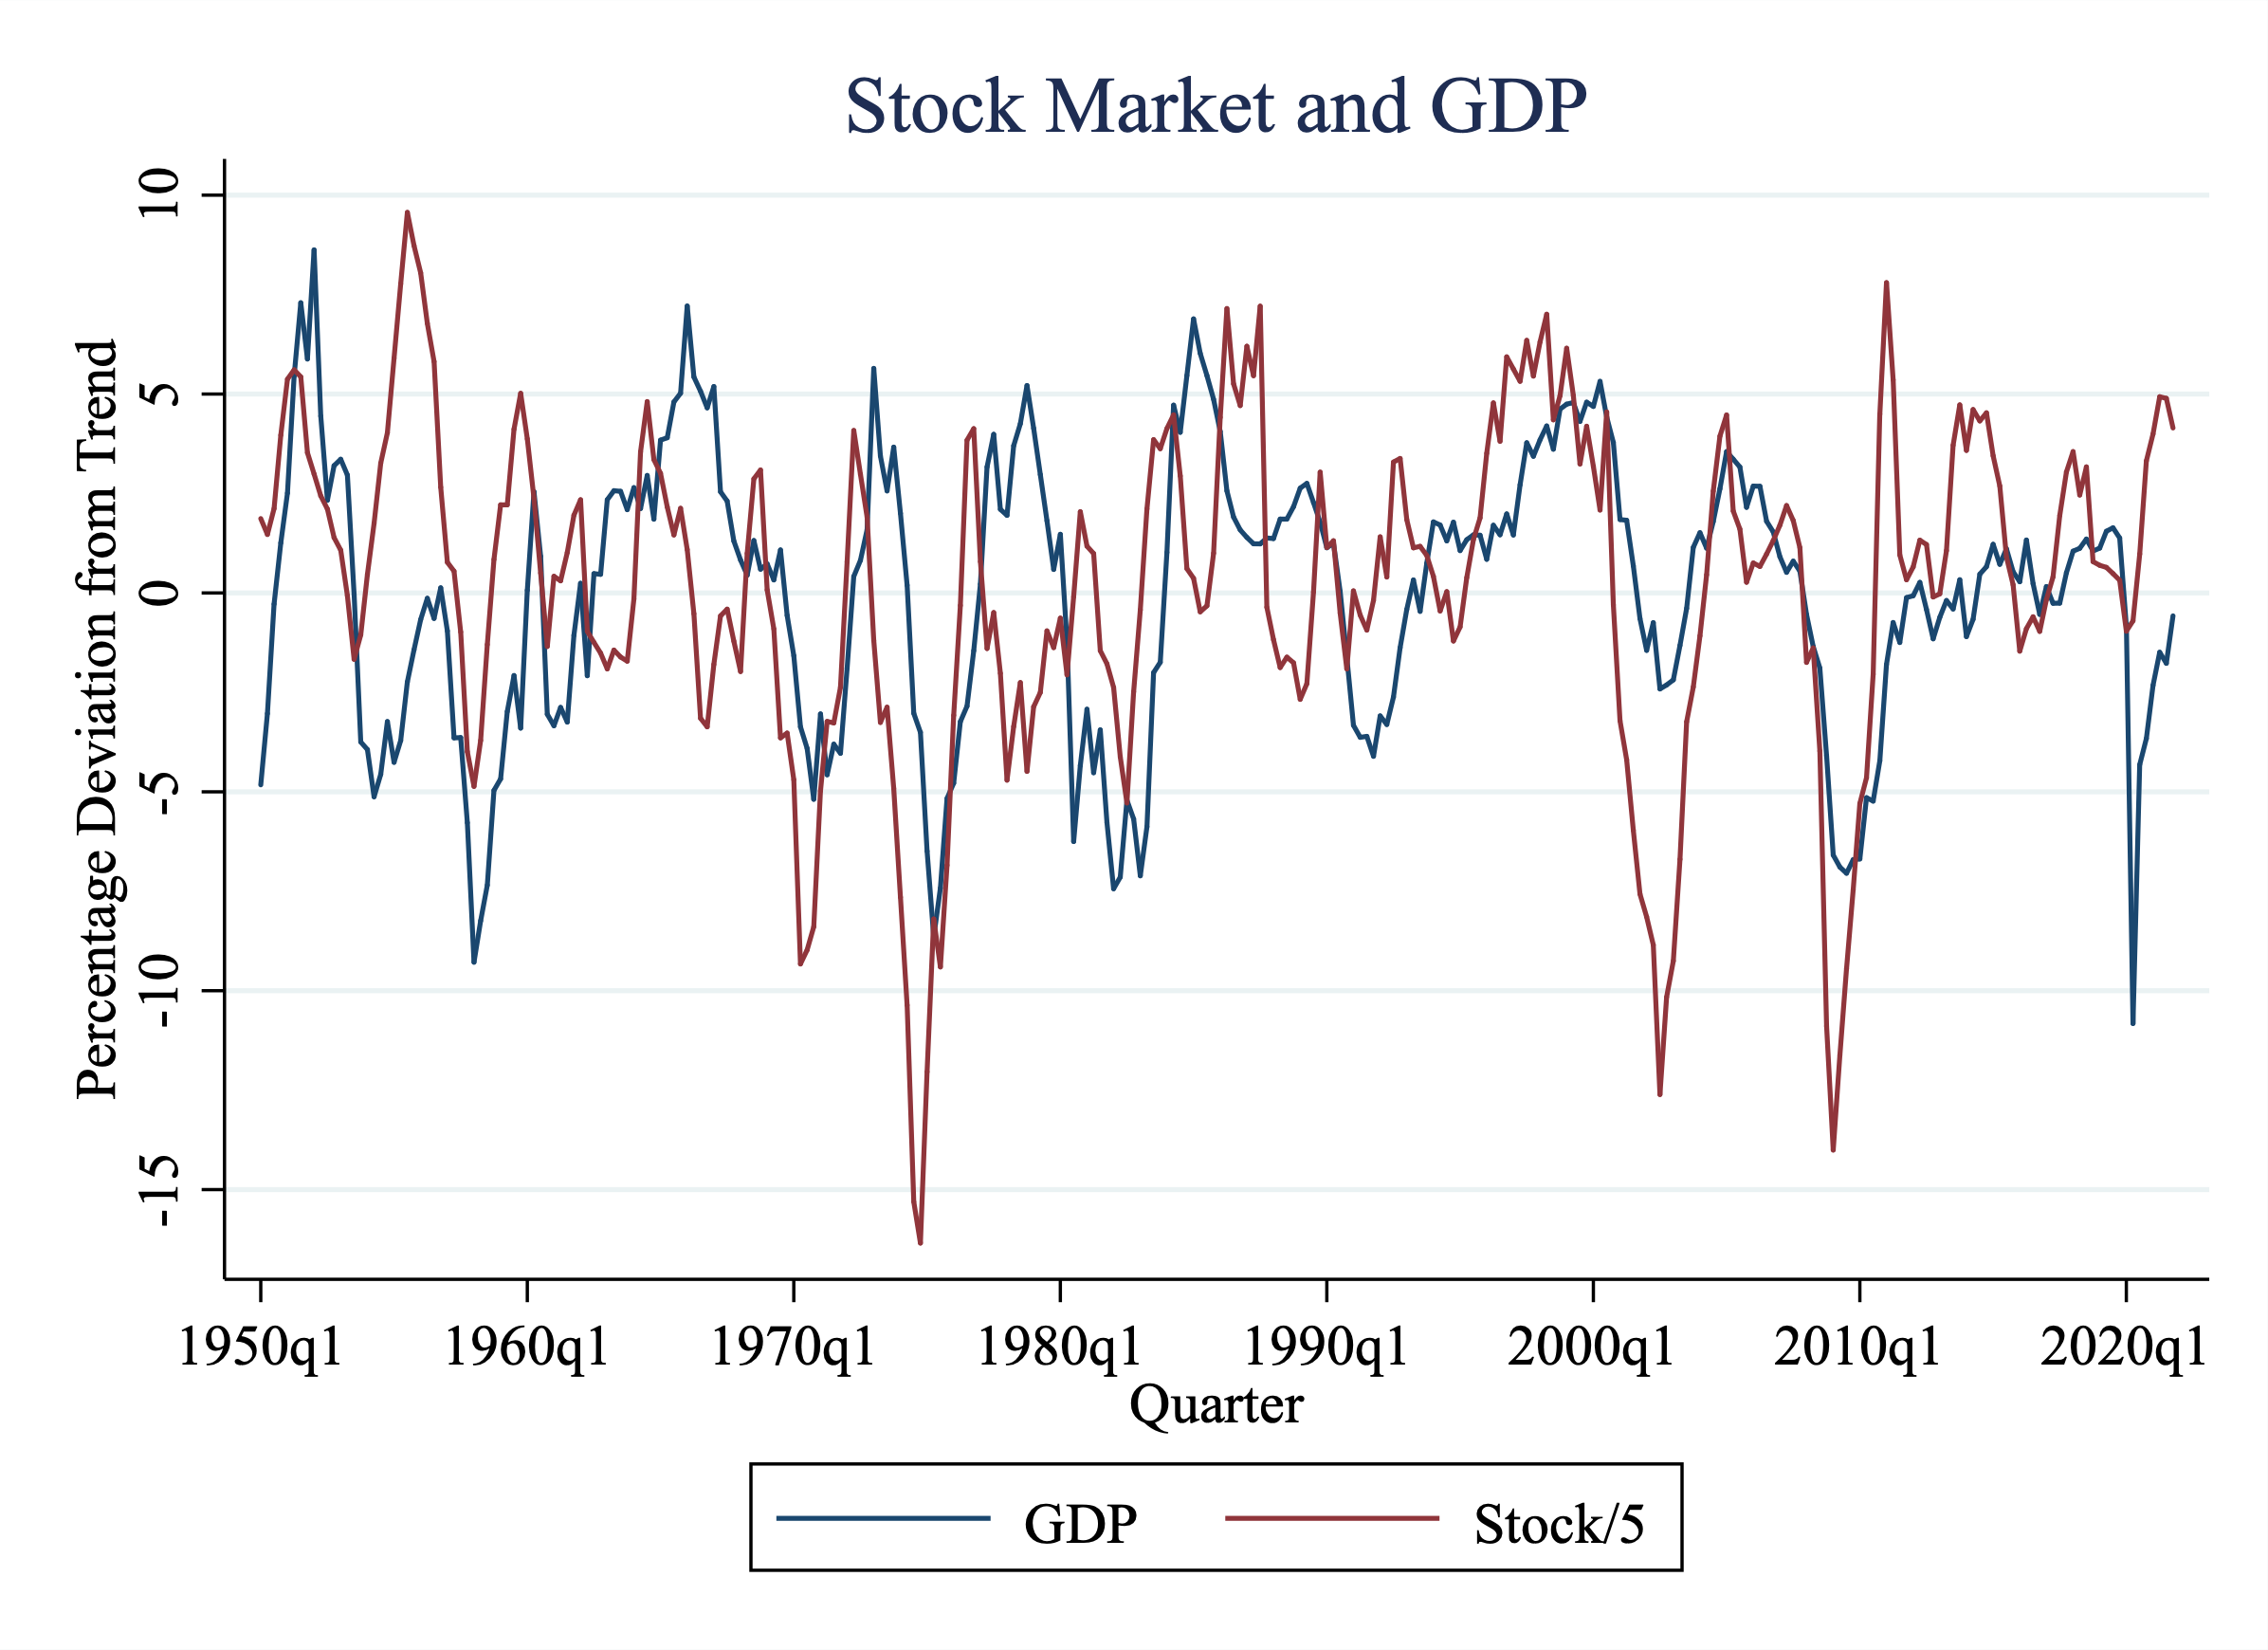
\includegraphics[scale=0.25]{Figures/StockvsGDP.png}
\end{figure}
\end{frame}



\begin{frame}
\frametitle[alignment=center]{Employment to Population Ratio}
\begin{figure}
\centering
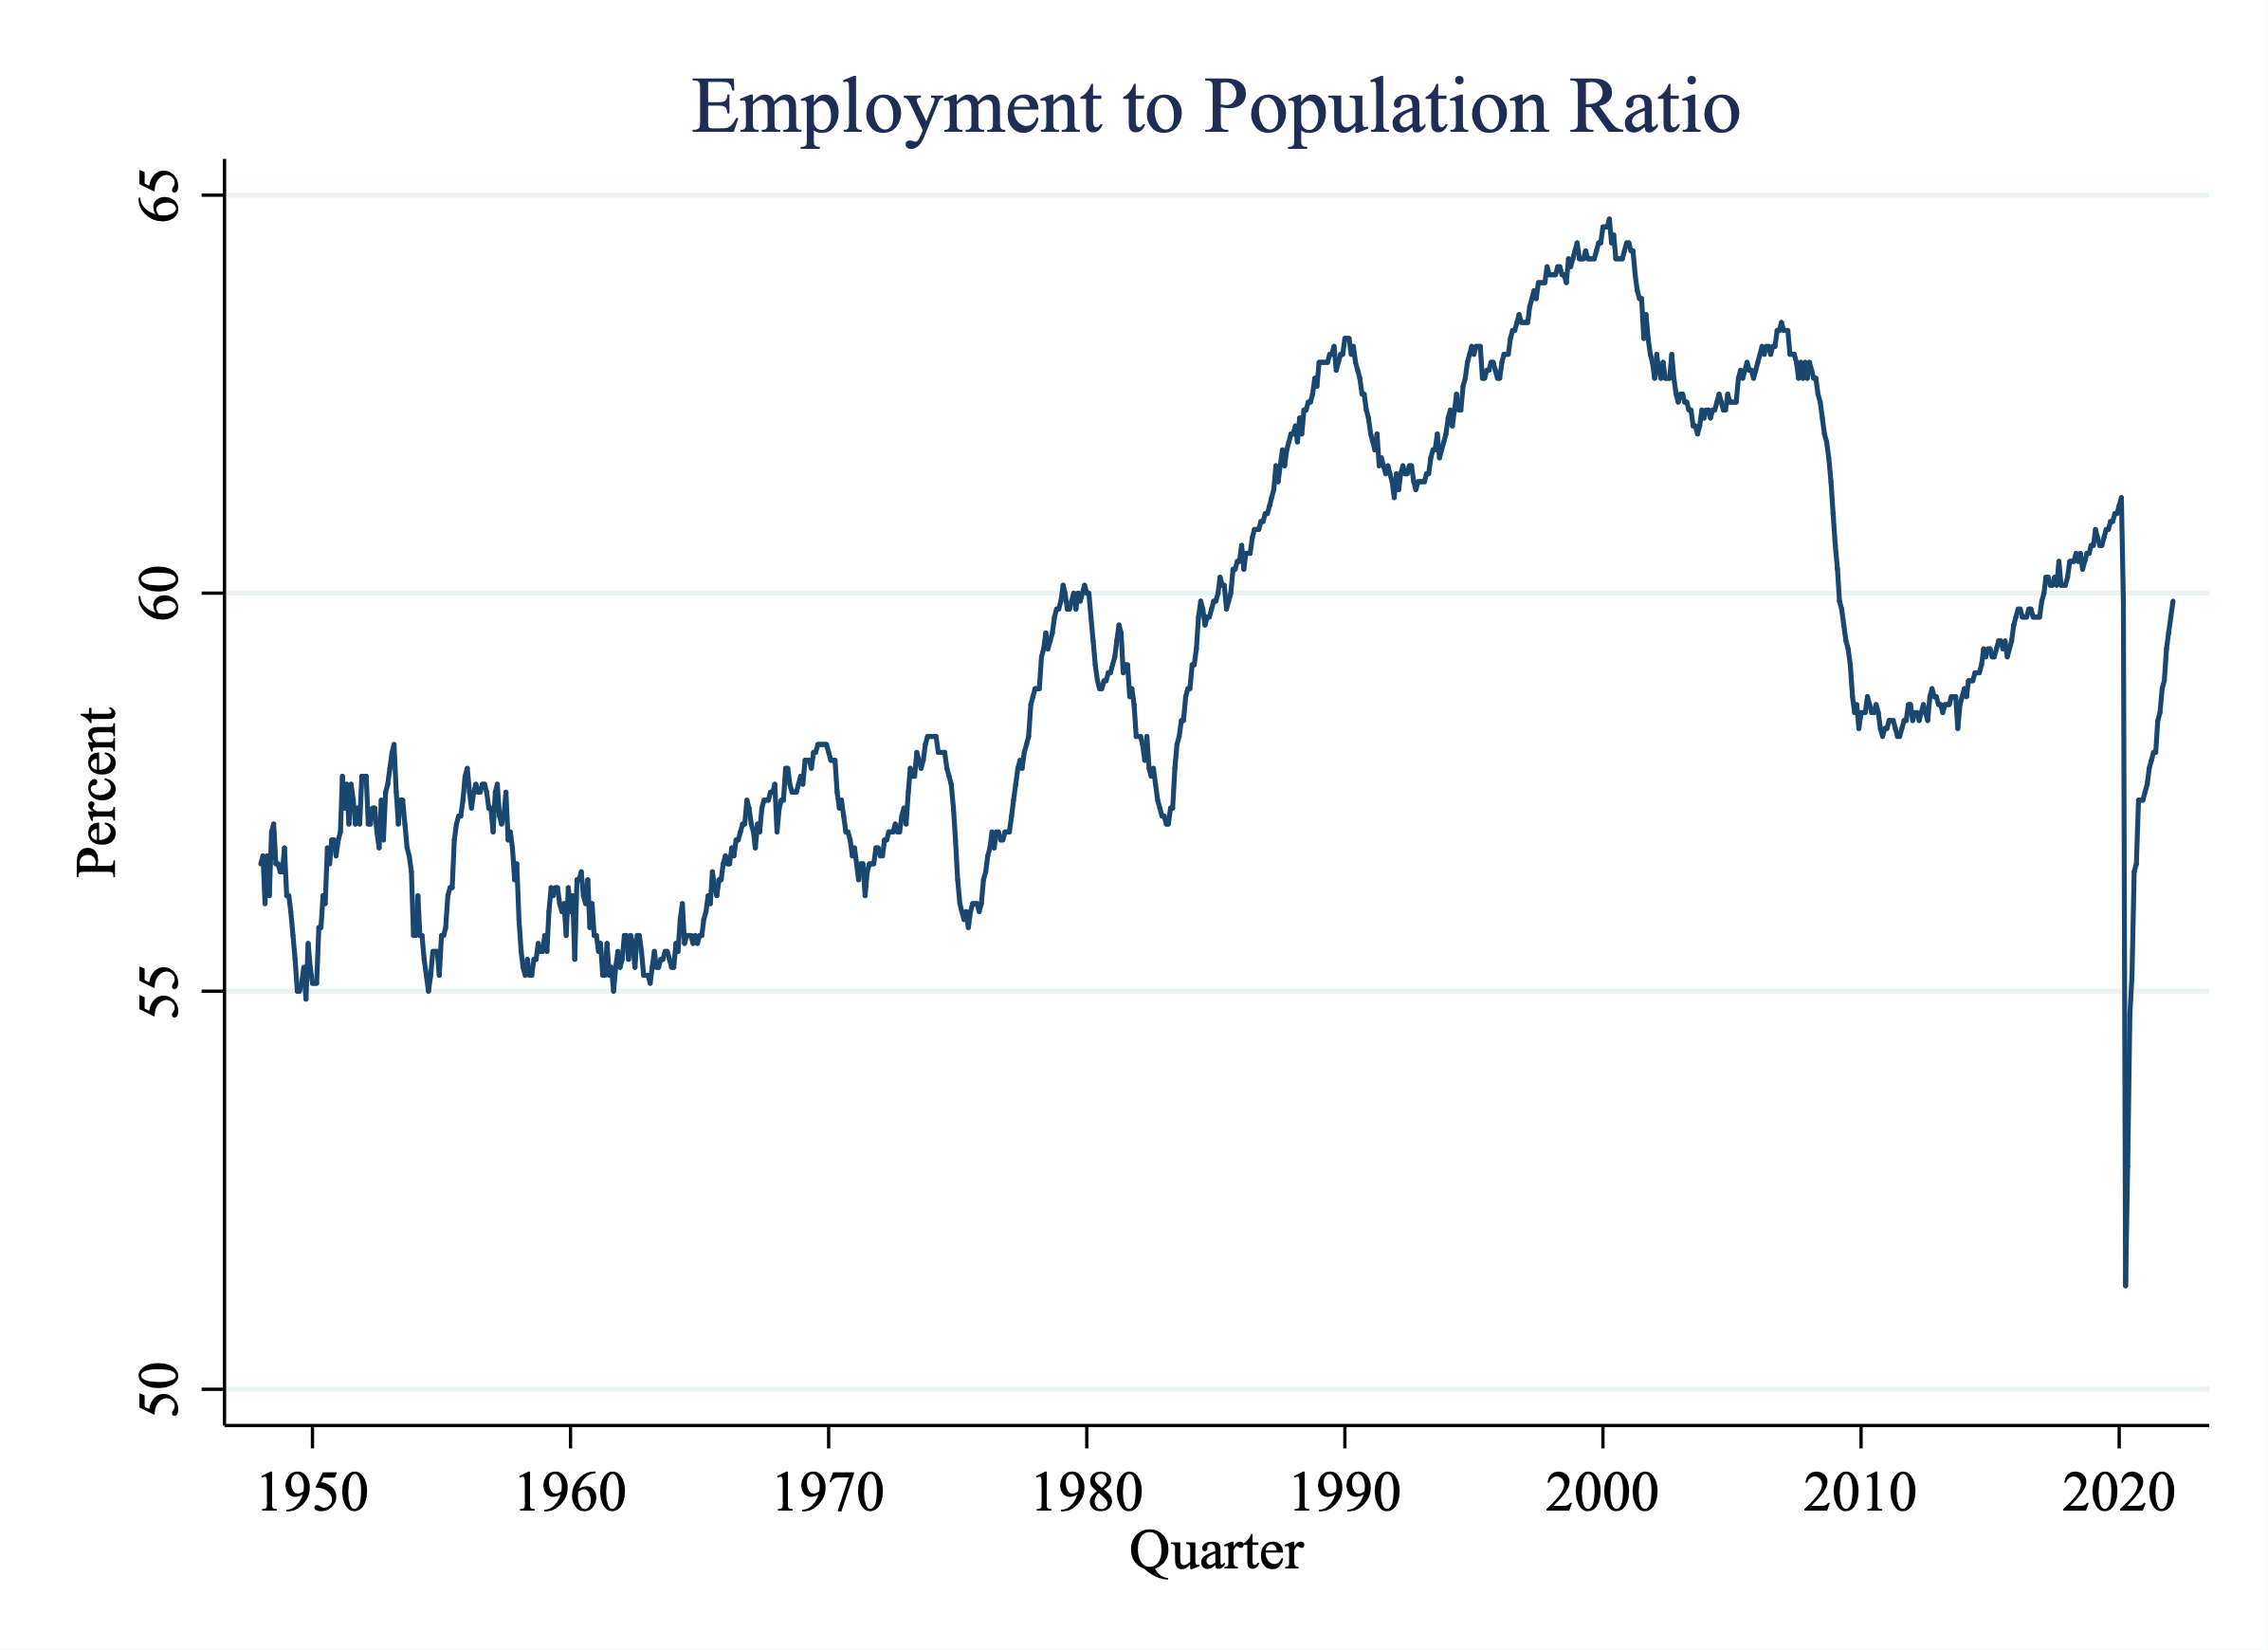
\includegraphics[scale=0.25]{Figures/EmPop1.png}
\end{figure}
\end{frame}

\begin{frame}
\frametitle[alignment=center]{Employment to Population Ratio-Men vs Women}
\begin{figure}
\centering
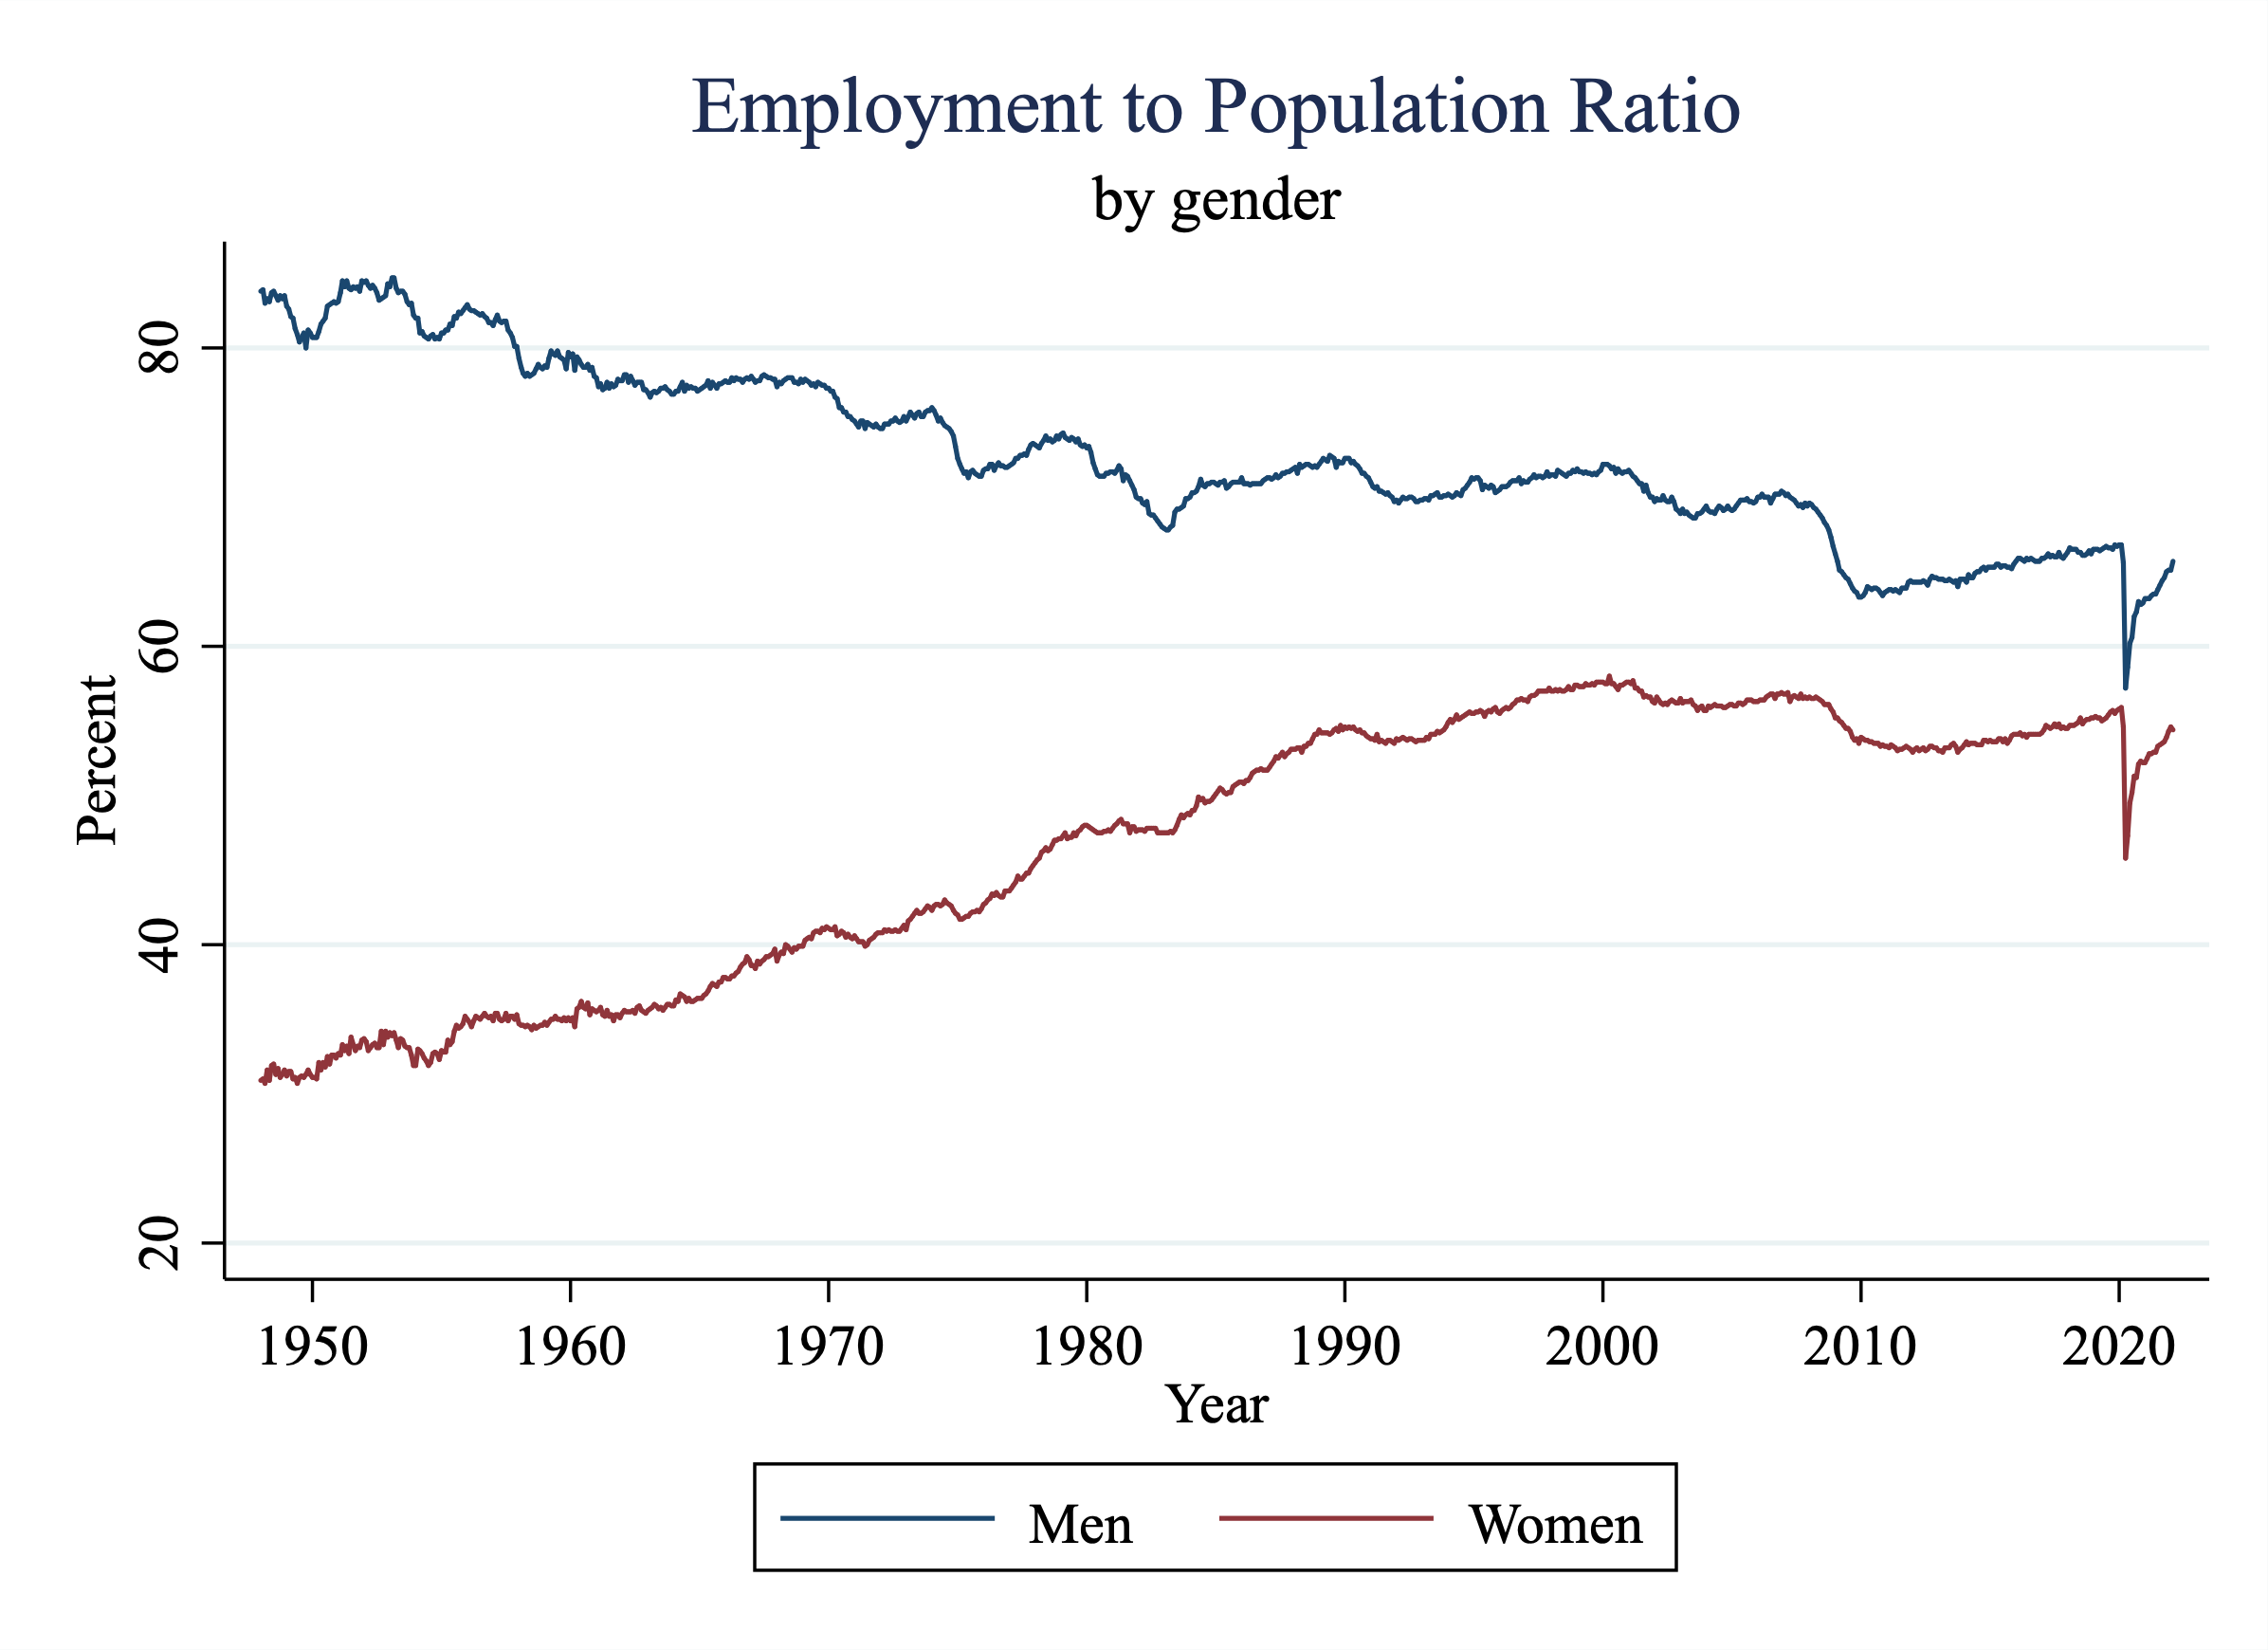
\includegraphics[scale=0.25]{Figures/EmPop2.png}
\end{figure}
\end{frame}

\begin{frame}
\frametitle[alignment=center]{Employment to Population Ratio-by Age}
\begin{figure}
\centering
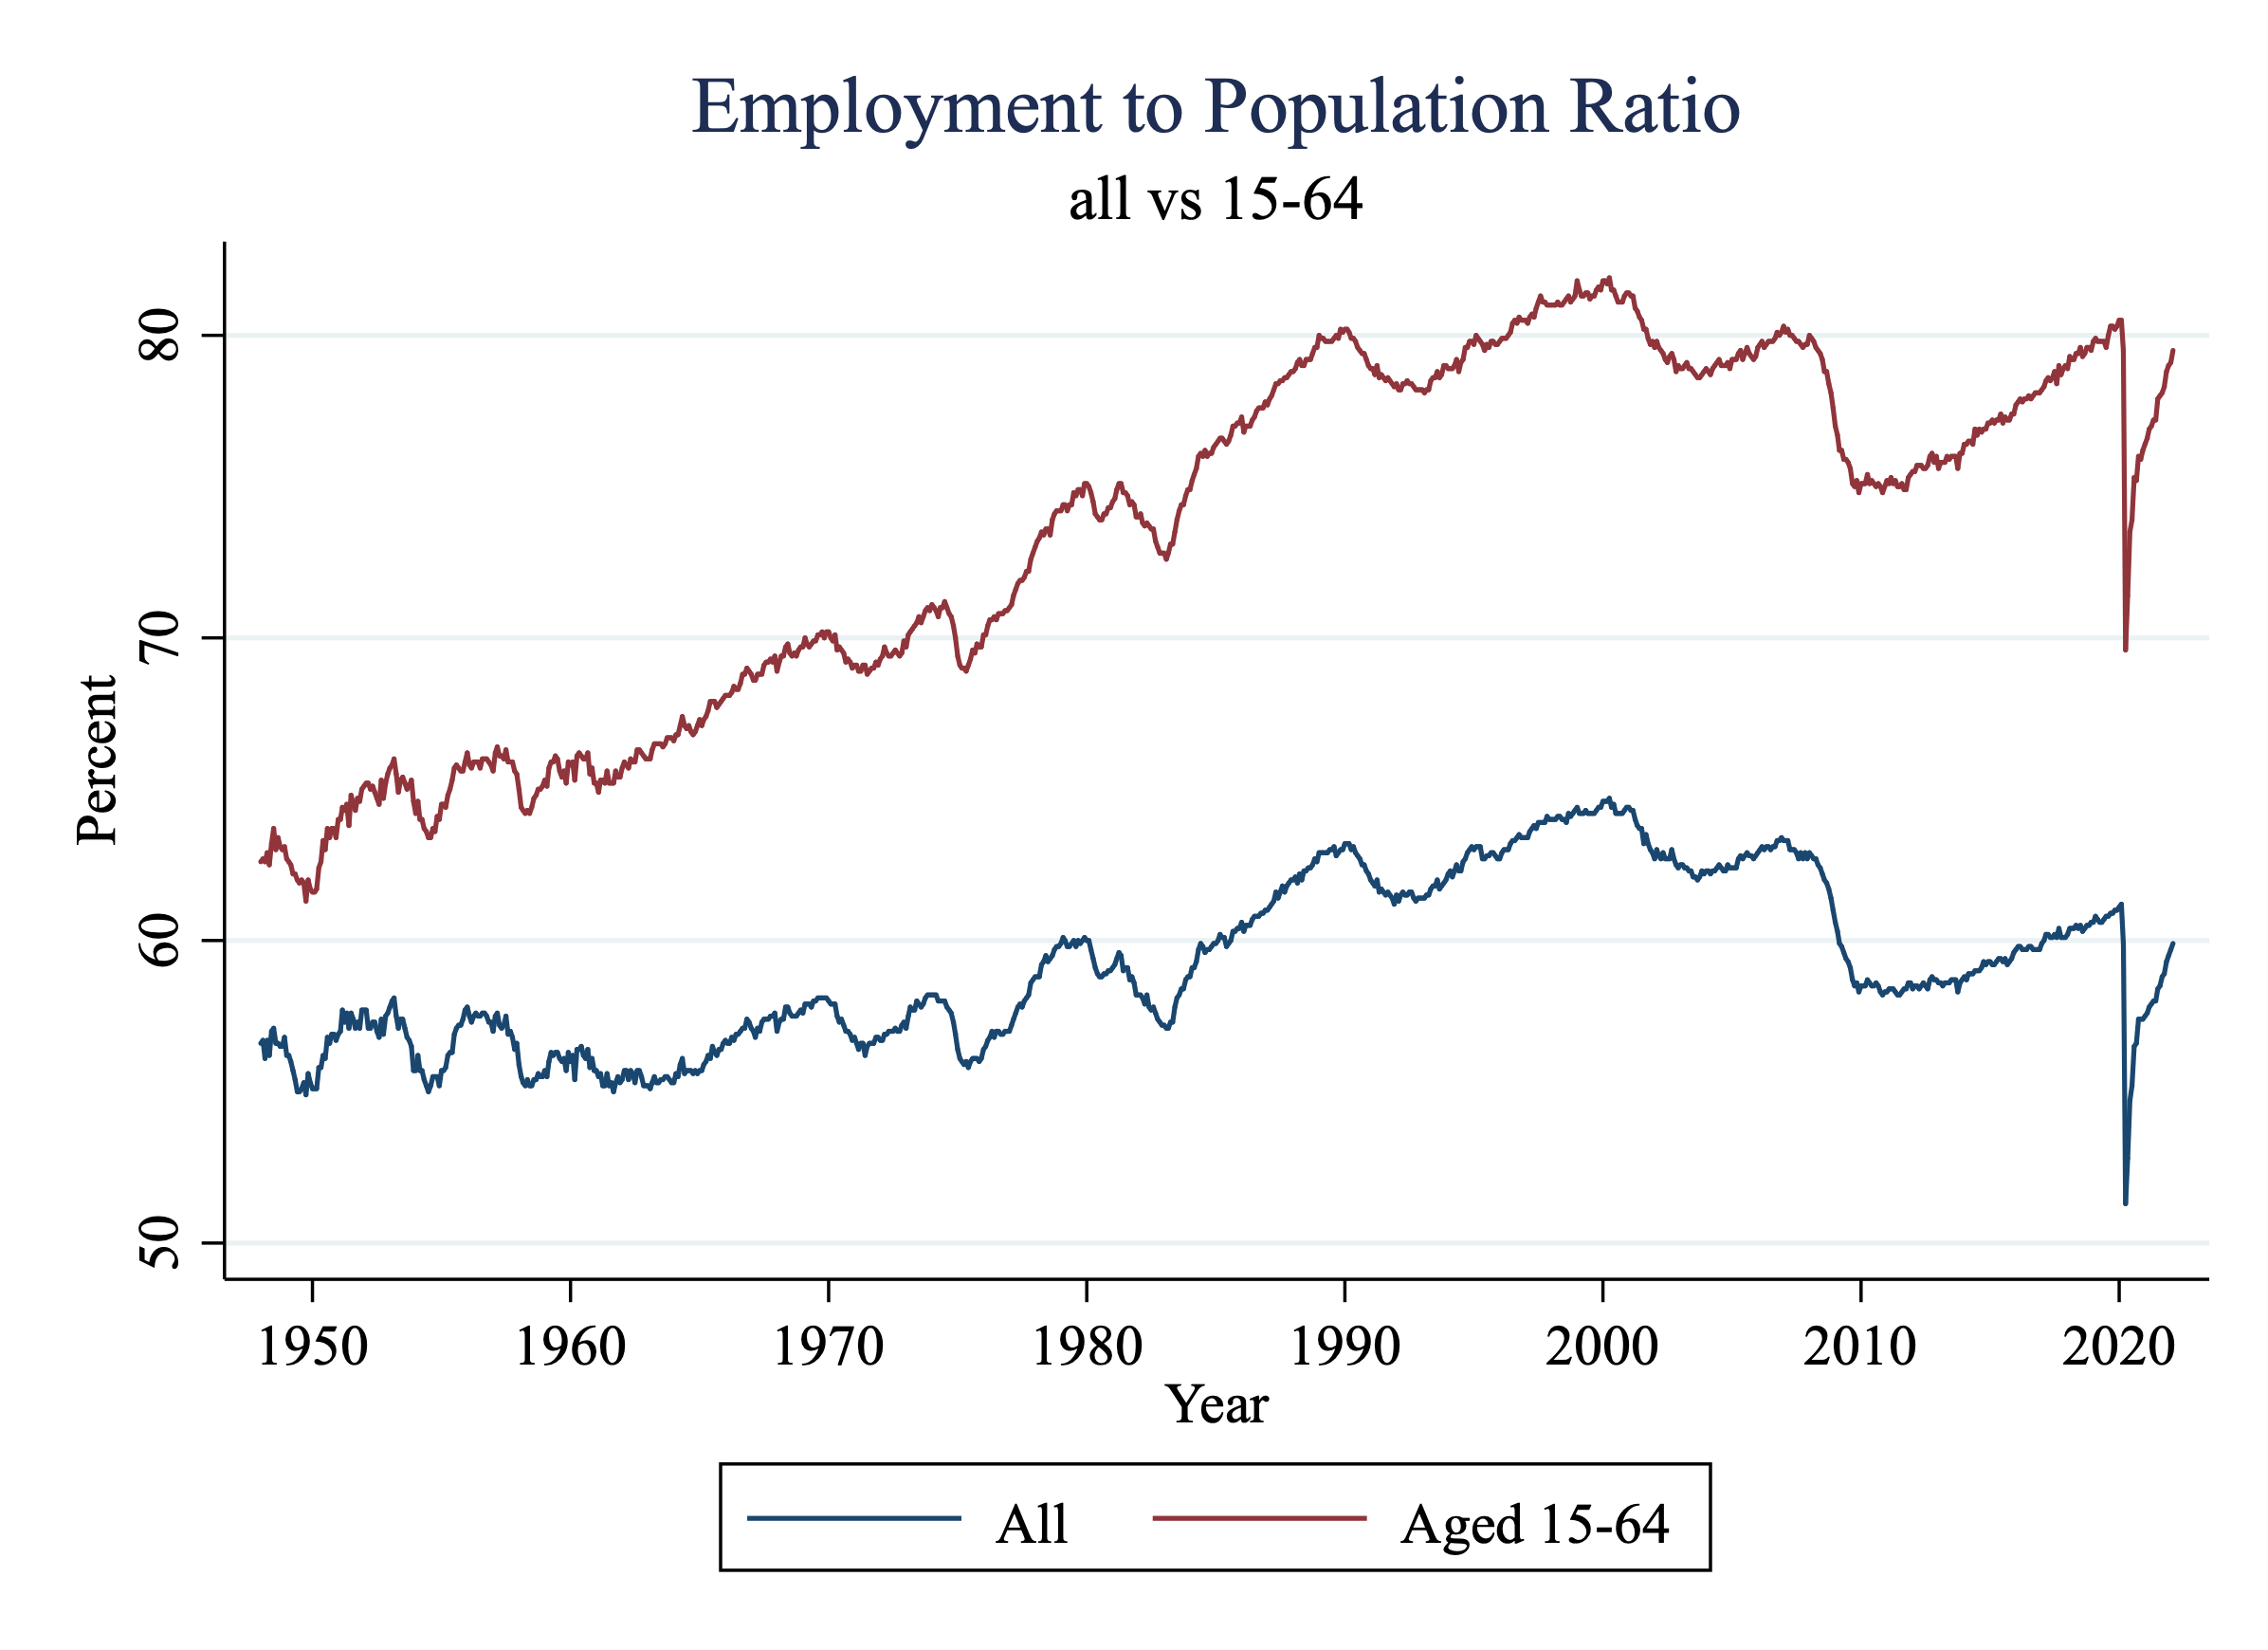
\includegraphics[scale=0.25]{Figures/EmPop3.png}
\end{figure}
\end{frame}

\begin{frame}
\frametitle[alignment=center]{Correlation Coefficients and Variability of Percentage Deviations from Trend}
\begin{table}
\centering
\begin{tabular}{lcc}
\hline\hline
Variable & Correlation & Standard Deviation \\
 & Coefficient & (\# of S.D. of GDP) \\
 \hline
Consumption & 0.89 & 0.87 \\
Investment  & 0.86 & 3.79 \\
Employment & 0.82  &. 1.22 \\ 
Average Labor Productivity & 0.31 & 0.63 \\
Housing & 0.43 & 7.97 \\
Price index & -0.23 & 0.94 \\
Stock index & 0.41 & 6.33 \\
\hline\hline
\end{tabular}
\end{table}
\end{frame}

\begin{frame}
\frametitle[alignment=center]{Summary of Business Cycle Facts}
\begin{table}
\centering
\begin{tabular}{llll}
\hline\hline
Variable & Cyclicality & Lead/Lag & Variation Rel.  \\
Variable & Cyclicality & Lead/Lag &  to GDP \\
\hline
Consumption & Procyclical & Coincident & Smaller \\
Investment & Procyclical & Coincident & Larger \\
Employment & Procyclical & Lagging & Smaller \\
Real Wage & Procyclical & (?) & (?) \\
 Avg Labor Productivity & Coincident & Smaller \\
\hline\hline
\end{tabular}
\end{table}
\end{frame}


\begin{frame}
\frametitle[alignment=center]{Selected Takeaways}
\begin{itemize}
\item We'll be building up a model to explain the time series of a bunch of facts \textbf{jointly}
\bigskip
\item How things move with GDP is how we organize thinking
\bigskip
\item Important facts to build up:  consumption and investment move with GDP, but consumption is less volatile and investment is much more volatile
\bigskip
\item Perhaps surprisingly to non-economists, the price level is \textbf{countercyclical}: prices are cyclically low in booms, and high in recessions\textcolor{red}{!}
\item Next:  we start to build our macroeconomy from microeconomic behaviors
\end{itemize}
\end{frame}



\end{document}